% Options for packages loaded elsewhere
\PassOptionsToPackage{unicode}{hyperref}
\PassOptionsToPackage{hyphens}{url}
%
\documentclass[
]{article}
\usepackage{lmodern}
\usepackage{amssymb,amsmath}
\usepackage{ifxetex,ifluatex}
\ifnum 0\ifxetex 1\fi\ifluatex 1\fi=0 % if pdftex
  \usepackage[T1]{fontenc}
  \usepackage[utf8]{inputenc}
  \usepackage{textcomp} % provide euro and other symbols
\else % if luatex or xetex
  \usepackage{unicode-math}
  \defaultfontfeatures{Scale=MatchLowercase}
  \defaultfontfeatures[\rmfamily]{Ligatures=TeX,Scale=1}
\fi
% Use upquote if available, for straight quotes in verbatim environments
\IfFileExists{upquote.sty}{\usepackage{upquote}}{}
\IfFileExists{microtype.sty}{% use microtype if available
  \usepackage[]{microtype}
  \UseMicrotypeSet[protrusion]{basicmath} % disable protrusion for tt fonts
}{}
\makeatletter
\@ifundefined{KOMAClassName}{% if non-KOMA class
  \IfFileExists{parskip.sty}{%
    \usepackage{parskip}
  }{% else
    \setlength{\parindent}{0pt}
    \setlength{\parskip}{6pt plus 2pt minus 1pt}}
}{% if KOMA class
  \KOMAoptions{parskip=half}}
\makeatother
\usepackage{xcolor}
\IfFileExists{xurl.sty}{\usepackage{xurl}}{} % add URL line breaks if available
\IfFileExists{bookmark.sty}{\usepackage{bookmark}}{\usepackage{hyperref}}
\hypersetup{
  pdftitle={Reallocation Rate Analysis with Interaction Term between Industry Category and Time},
  hidelinks,
  pdfcreator={LaTeX via pandoc}}
\urlstyle{same} % disable monospaced font for URLs
\usepackage[margin=1in]{geometry}
\usepackage{color}
\usepackage{fancyvrb}
\newcommand{\VerbBar}{|}
\newcommand{\VERB}{\Verb[commandchars=\\\{\}]}
\DefineVerbatimEnvironment{Highlighting}{Verbatim}{commandchars=\\\{\}}
% Add ',fontsize=\small' for more characters per line
\usepackage{framed}
\definecolor{shadecolor}{RGB}{248,248,248}
\newenvironment{Shaded}{\begin{snugshade}}{\end{snugshade}}
\newcommand{\AlertTok}[1]{\textcolor[rgb]{0.94,0.16,0.16}{#1}}
\newcommand{\AnnotationTok}[1]{\textcolor[rgb]{0.56,0.35,0.01}{\textbf{\textit{#1}}}}
\newcommand{\AttributeTok}[1]{\textcolor[rgb]{0.77,0.63,0.00}{#1}}
\newcommand{\BaseNTok}[1]{\textcolor[rgb]{0.00,0.00,0.81}{#1}}
\newcommand{\BuiltInTok}[1]{#1}
\newcommand{\CharTok}[1]{\textcolor[rgb]{0.31,0.60,0.02}{#1}}
\newcommand{\CommentTok}[1]{\textcolor[rgb]{0.56,0.35,0.01}{\textit{#1}}}
\newcommand{\CommentVarTok}[1]{\textcolor[rgb]{0.56,0.35,0.01}{\textbf{\textit{#1}}}}
\newcommand{\ConstantTok}[1]{\textcolor[rgb]{0.00,0.00,0.00}{#1}}
\newcommand{\ControlFlowTok}[1]{\textcolor[rgb]{0.13,0.29,0.53}{\textbf{#1}}}
\newcommand{\DataTypeTok}[1]{\textcolor[rgb]{0.13,0.29,0.53}{#1}}
\newcommand{\DecValTok}[1]{\textcolor[rgb]{0.00,0.00,0.81}{#1}}
\newcommand{\DocumentationTok}[1]{\textcolor[rgb]{0.56,0.35,0.01}{\textbf{\textit{#1}}}}
\newcommand{\ErrorTok}[1]{\textcolor[rgb]{0.64,0.00,0.00}{\textbf{#1}}}
\newcommand{\ExtensionTok}[1]{#1}
\newcommand{\FloatTok}[1]{\textcolor[rgb]{0.00,0.00,0.81}{#1}}
\newcommand{\FunctionTok}[1]{\textcolor[rgb]{0.00,0.00,0.00}{#1}}
\newcommand{\ImportTok}[1]{#1}
\newcommand{\InformationTok}[1]{\textcolor[rgb]{0.56,0.35,0.01}{\textbf{\textit{#1}}}}
\newcommand{\KeywordTok}[1]{\textcolor[rgb]{0.13,0.29,0.53}{\textbf{#1}}}
\newcommand{\NormalTok}[1]{#1}
\newcommand{\OperatorTok}[1]{\textcolor[rgb]{0.81,0.36,0.00}{\textbf{#1}}}
\newcommand{\OtherTok}[1]{\textcolor[rgb]{0.56,0.35,0.01}{#1}}
\newcommand{\PreprocessorTok}[1]{\textcolor[rgb]{0.56,0.35,0.01}{\textit{#1}}}
\newcommand{\RegionMarkerTok}[1]{#1}
\newcommand{\SpecialCharTok}[1]{\textcolor[rgb]{0.00,0.00,0.00}{#1}}
\newcommand{\SpecialStringTok}[1]{\textcolor[rgb]{0.31,0.60,0.02}{#1}}
\newcommand{\StringTok}[1]{\textcolor[rgb]{0.31,0.60,0.02}{#1}}
\newcommand{\VariableTok}[1]{\textcolor[rgb]{0.00,0.00,0.00}{#1}}
\newcommand{\VerbatimStringTok}[1]{\textcolor[rgb]{0.31,0.60,0.02}{#1}}
\newcommand{\WarningTok}[1]{\textcolor[rgb]{0.56,0.35,0.01}{\textbf{\textit{#1}}}}
\usepackage{graphicx,grffile}
\makeatletter
\def\maxwidth{\ifdim\Gin@nat@width>\linewidth\linewidth\else\Gin@nat@width\fi}
\def\maxheight{\ifdim\Gin@nat@height>\textheight\textheight\else\Gin@nat@height\fi}
\makeatother
% Scale images if necessary, so that they will not overflow the page
% margins by default, and it is still possible to overwrite the defaults
% using explicit options in \includegraphics[width, height, ...]{}
\setkeys{Gin}{width=\maxwidth,height=\maxheight,keepaspectratio}
% Set default figure placement to htbp
\makeatletter
\def\fps@figure{htbp}
\makeatother
\setlength{\emergencystretch}{3em} % prevent overfull lines
\providecommand{\tightlist}{%
  \setlength{\itemsep}{0pt}\setlength{\parskip}{0pt}}
\setcounter{secnumdepth}{-\maxdimen} % remove section numbering

\title{Reallocation Rate Analysis with Interaction Term between Industry
Category and Time}
\author{}
\date{\vspace{-2.5em}}

\begin{document}
\maketitle

The general regression model used in analyzing the effects of different
training indices on different reallocation rates is as follow:

\[R_j = \alpha + \beta T_i + \gamma t + \sum_n \delta I_n + \sum_n \lambda_n I_n t\]

\begin{itemize}
\tightlist
\item
  \(R =\) \emph{Reallocation Rate}
\item
  \(j =\) \emph{Type of reallocation rate }
\item
  \(T =\) \emph{Training Index}
\item
  \(i =\) \emph{type of training index}
\item
  \(t =\) \emph{time, treated as a continuous variable with 2004 denoted
  as 1 and 2018 denoted as 15 }
\item
  \(I =\) \emph{industry}
\item
  \(n =\) \emph{type of industry based on NAICS Classification}
\end{itemize}

\hypertarget{job-reallocation-rate}{%
\section{Job Reallocation Rate}\label{job-reallocation-rate}}

Job Reallocation Rate refers to total jobs created plus total jobs
destroyed, divided by total jobs in the economy. This measure allows us
to look at how quickly jobs are reallocated from shrinking firms to
expanding ones.

The data source for job reallocation is from the Business Employment
Dynamics which collects quarterly job creation and destruction of firms.

Job Reallocation \textbf{does not} include workers switching jobs if the
job is not created or destroyed.

\hypertarget{results}{%
\subsection{Results}\label{results}}

\hypertarget{in-planton-site-training-pt}{%
\subsubsection{In-Plant/On-Site Training
(PT)}\label{in-planton-site-training-pt}}

\begin{Shaded}
\begin{Highlighting}[]
\NormalTok{lmod <-}\StringTok{ }\KeywordTok{lm}\NormalTok{(adj_realloc }\OperatorTok{~}\StringTok{  }\NormalTok{PT }\OperatorTok{+}\StringTok{ }\NormalTok{industryCategory}\OperatorTok{*}\NormalTok{period.num, t)}
\KeywordTok{summary}\NormalTok{(lmod)}
\end{Highlighting}
\end{Shaded}

\begin{verbatim}
## 
## Call:
## lm(formula = adj_realloc ~ PT + industryCategory * period.num, 
##     data = t)
## 
## Residuals:
##      Min       1Q   Median       3Q      Max 
## -1.54762 -0.27447 -0.00989  0.22250  2.17376 
## 
## Coefficients:
##                                Estimate Std. Error t value Pr(>|t|)    
## (Intercept)                    44.53581    5.89793   7.551 8.43e-13 ***
## PT                              0.06106    1.96107   0.031    0.975    
## industryCategory21            -33.23786    1.20054 -27.686  < 2e-16 ***
## industryCategory22            -39.72003    1.92276 -20.658  < 2e-16 ***
## industryCategory23            -20.31841    2.48105  -8.189 1.43e-14 ***
## industryCategory31            -36.04279    0.79409 -45.389  < 2e-16 ***
## industryCategory42            -33.55651    0.59608 -56.295  < 2e-16 ***
## industryCategory44            -30.93434    0.57492 -53.806  < 2e-16 ***
## industryCategory48            -33.17344    0.47614 -69.671  < 2e-16 ***
## industryCategory51            -35.03275    0.69161 -50.654  < 2e-16 ***
## industryCategory52            -34.71379    0.49439 -70.216  < 2e-16 ***
## industryCategory53            -29.08317    0.59324 -49.025  < 2e-16 ***
## industryCategory54            -29.62746    0.87098 -34.016  < 2e-16 ***
## industryCategory55            -37.34222    0.76835 -48.600  < 2e-16 ***
## industryCategory56            -25.07805    0.48882 -51.303  < 2e-16 ***
## industryCategory61            -31.14762    0.60537 -51.452  < 2e-16 ***
## industryCategory62            -36.26562    0.66390 -54.625  < 2e-16 ***
## industryCategory71            -15.01751    0.66650 -22.532  < 2e-16 ***
## industryCategory72            -28.23789    1.35131 -20.897  < 2e-16 ***
## industryCategory81            -28.87834    0.47255 -61.112  < 2e-16 ***
## period.num                     -0.65205    0.03484 -18.714  < 2e-16 ***
## industryCategory21:period.num   0.69764    0.04941  14.119  < 2e-16 ***
## industryCategory22:period.num   0.59975    0.04977  12.051  < 2e-16 ***
## industryCategory23:period.num   0.33045    0.04933   6.698 1.42e-10 ***
## industryCategory31:period.num   0.49072    0.04924   9.965  < 2e-16 ***
## industryCategory42:period.num   0.48628    0.04912   9.901  < 2e-16 ***
## industryCategory44:period.num   0.47130    0.04911   9.596  < 2e-16 ***
## industryCategory48:period.num   0.57725    0.04915  11.745  < 2e-16 ***
## industryCategory51:period.num   0.69505    0.04957  14.022  < 2e-16 ***
## industryCategory52:period.num   0.45541    0.05008   9.094  < 2e-16 ***
## industryCategory53:period.num   0.46047    0.05057   9.105  < 2e-16 ***
## industryCategory54:period.num   0.45040    0.05015   8.981  < 2e-16 ***
## industryCategory55:period.num   0.55988    0.04912  11.398  < 2e-16 ***
## industryCategory56:period.num   0.42644    0.04939   8.634 7.56e-16 ***
## industryCategory61:period.num   0.58767    0.04911  11.966  < 2e-16 ***
## industryCategory62:period.num   0.58633    0.05313  11.036  < 2e-16 ***
## industryCategory71:period.num   0.43091    0.04919   8.760 3.22e-16 ***
## industryCategory72:period.num   0.50023    0.04948  10.109  < 2e-16 ***
## industryCategory81:period.num   0.50409    0.04913  10.261  < 2e-16 ***
## ---
## Signif. codes:  0 '***' 0.001 '**' 0.01 '*' 0.05 '.' 0.1 ' ' 1
## 
## Residual standard error: 0.5811 on 246 degrees of freedom
## Multiple R-squared:  0.9956, Adjusted R-squared:  0.9949 
## F-statistic:  1453 on 38 and 246 DF,  p-value: < 2.2e-16
\end{verbatim}

\hypertarget{on-the-job-training-oj}{%
\subsubsection{On-the-Job Training (OJ)}\label{on-the-job-training-oj}}

\begin{Shaded}
\begin{Highlighting}[]
\NormalTok{lmod <-}\StringTok{ }\KeywordTok{lm}\NormalTok{(adj_realloc }\OperatorTok{~}\StringTok{  }\NormalTok{OJ }\OperatorTok{+}\StringTok{ }\NormalTok{industryCategory}\OperatorTok{*}\NormalTok{period.num, t)}
\KeywordTok{summary}\NormalTok{(lmod)}
\end{Highlighting}
\end{Shaded}

\begin{verbatim}
## 
## Call:
## lm(formula = adj_realloc ~ OJ + industryCategory * period.num, 
##     data = t)
## 
## Residuals:
##      Min       1Q   Median       3Q      Max 
## -1.51901 -0.27265 -0.01241  0.22898  2.21033 
## 
## Coefficients:
##                                Estimate Std. Error t value Pr(>|t|)    
## (Intercept)                    53.03502    8.44533   6.280 1.52e-09 ***
## OJ                             -2.54083    2.57860  -0.985    0.325    
## industryCategory21            -31.28610    1.99595 -15.675  < 2e-16 ***
## industryCategory22            -36.62121    3.11779 -11.746  < 2e-16 ***
## industryCategory23            -16.81400    3.50781  -4.793 2.84e-06 ***
## industryCategory31            -34.86083    1.26021 -27.663  < 2e-16 ***
## industryCategory42            -33.09353    0.63861 -51.822  < 2e-16 ***
## industryCategory44            -31.36493    0.61620 -50.901  < 2e-16 ***
## industryCategory48            -33.11469    0.44897 -73.758  < 2e-16 ***
## industryCategory51            -34.22974    0.91423 -37.441  < 2e-16 ***
## industryCategory52            -34.04918    0.80284 -42.411  < 2e-16 ***
## industryCategory53            -28.15372    1.03210 -27.278  < 2e-16 ***
## industryCategory54            -27.94672    1.74013 -16.060  < 2e-16 ***
## industryCategory55            -36.18894    1.23396 -29.328  < 2e-16 ***
## industryCategory56            -25.39281    0.54469 -46.619  < 2e-16 ***
## industryCategory61            -30.61463    0.69094 -44.309  < 2e-16 ***
## industryCategory62            -36.65890    0.58801 -62.344  < 2e-16 ***
## industryCategory71            -15.81278    0.90831 -17.409  < 2e-16 ***
## industryCategory72            -30.16335    1.96499 -15.350  < 2e-16 ***
## industryCategory81            -28.29836    0.73439 -38.533  < 2e-16 ***
## period.num                     -0.65101    0.03467 -18.776  < 2e-16 ***
## industryCategory21:period.num   0.70814    0.05020  14.107  < 2e-16 ***
## industryCategory22:period.num   0.61865    0.05255  11.774  < 2e-16 ***
## industryCategory23:period.num   0.32869    0.04904   6.702 1.39e-10 ***
## industryCategory31:period.num   0.50657    0.05155   9.826  < 2e-16 ***
## industryCategory42:period.num   0.49452    0.04972   9.946  < 2e-16 ***
## industryCategory44:period.num   0.47319    0.04905   9.646  < 2e-16 ***
## industryCategory48:period.num   0.57099    0.04942  11.554  < 2e-16 ***
## industryCategory51:period.num   0.72470    0.05763  12.575  < 2e-16 ***
## industryCategory52:period.num   0.48292    0.05626   8.584 1.05e-15 ***
## industryCategory53:period.num   0.47867    0.05225   9.161  < 2e-16 ***
## industryCategory54:period.num   0.46446    0.05114   9.082  < 2e-16 ***
## industryCategory55:period.num   0.58635    0.05588  10.493  < 2e-16 ***
## industryCategory56:period.num   0.43571    0.04988   8.735 3.82e-16 ***
## industryCategory61:period.num   0.59709    0.04994  11.957  < 2e-16 ***
## industryCategory62:period.num   0.58037    0.04947  11.732  < 2e-16 ***
## industryCategory71:period.num   0.43733    0.04944   8.846  < 2e-16 ***
## industryCategory72:period.num   0.49825    0.04905  10.158  < 2e-16 ***
## industryCategory81:period.num   0.50731    0.04913  10.326  < 2e-16 ***
## ---
## Signif. codes:  0 '***' 0.001 '**' 0.01 '*' 0.05 '.' 0.1 ' ' 1
## 
## Residual standard error: 0.58 on 246 degrees of freedom
## Multiple R-squared:  0.9956, Adjusted R-squared:  0.9949 
## F-statistic:  1459 on 38 and 246 DF,  p-value: < 2.2e-16
\end{verbatim}

\hypertarget{relevant-work-experience-rw}{%
\subsubsection{Relevant Work Experience
(RW)}\label{relevant-work-experience-rw}}

\begin{Shaded}
\begin{Highlighting}[]
\NormalTok{lmod <-}\StringTok{ }\KeywordTok{lm}\NormalTok{(adj_realloc }\OperatorTok{~}\StringTok{  }\NormalTok{RW }\OperatorTok{+}\StringTok{ }\NormalTok{industryCategory}\OperatorTok{*}\NormalTok{period.num, t)}
\KeywordTok{summary}\NormalTok{(lmod)}
\end{Highlighting}
\end{Shaded}

\begin{verbatim}
## 
## Call:
## lm(formula = adj_realloc ~ RW + industryCategory * period.num, 
##     data = t)
## 
## Residuals:
##      Min       1Q   Median       3Q      Max 
## -1.57232 -0.26458 -0.00861  0.22651  2.16178 
## 
## Coefficients:
##                                Estimate Std. Error t value Pr(>|t|)    
## (Intercept)                    38.97068    5.85936   6.651 1.87e-10 ***
## RW                              1.34866    1.37267   0.983    0.327    
## industryCategory21            -34.72519    1.61196 -21.542  < 2e-16 ***
## industryCategory22            -41.86377    2.28507 -18.321  < 2e-16 ***
## industryCategory23            -22.28104    2.12225 -10.499  < 2e-16 ***
## industryCategory31            -37.23427    1.31155 -28.389  < 2e-16 ***
## industryCategory42            -35.25878    1.80111 -19.576  < 2e-16 ***
## industryCategory44            -30.76849    0.48075 -64.002  < 2e-16 ***
## industryCategory48            -33.44637    0.52794 -63.352  < 2e-16 ***
## industryCategory51            -37.00331    2.07092 -17.868  < 2e-16 ***
## industryCategory52            -36.15631    1.54080 -23.466  < 2e-16 ***
## industryCategory53            -30.11113    1.14864 -26.215  < 2e-16 ***
## industryCategory54            -32.25678    2.73638 -11.788  < 2e-16 ***
## industryCategory55            -39.92414    2.68497 -14.870  < 2e-16 ***
## industryCategory56            -25.28737    0.49129 -51.472  < 2e-16 ***
## industryCategory61            -32.22607    1.19669 -26.929  < 2e-16 ***
## industryCategory62            -36.51725    0.50643 -72.107  < 2e-16 ***
## industryCategory71            -15.34083    0.54483 -28.157  < 2e-16 ***
## industryCategory72            -27.21590    1.16890 -23.283  < 2e-16 ***
## industryCategory81            -29.80966    1.05188 -28.339  < 2e-16 ***
## period.num                     -0.65028    0.03470 -18.739  < 2e-16 ***
## industryCategory21:period.num   0.68067    0.05191  13.112  < 2e-16 ***
## industryCategory22:period.num   0.57878    0.05356  10.806  < 2e-16 ***
## industryCategory23:period.num   0.32008    0.05011   6.388 8.34e-10 ***
## industryCategory31:period.num   0.47423    0.05185   9.147  < 2e-16 ***
## industryCategory42:period.num   0.47521    0.05030   9.448  < 2e-16 ***
## industryCategory44:period.num   0.46900    0.04907   9.557  < 2e-16 ***
## industryCategory48:period.num   0.57269    0.04923  11.633  < 2e-16 ***
## industryCategory51:period.num   0.66472    0.05781  11.498  < 2e-16 ***
## industryCategory52:period.num   0.43707    0.05256   8.315 6.27e-15 ***
## industryCategory53:period.num   0.44786    0.05077   8.822  < 2e-16 ***
## industryCategory54:period.num   0.42546    0.05506   7.728 2.78e-13 ***
## industryCategory55:period.num   0.52031    0.06346   8.199 1.35e-14 ***
## industryCategory56:period.num   0.41428    0.05059   8.188 1.44e-14 ***
## industryCategory61:period.num   0.57576    0.05050  11.402  < 2e-16 ***
## industryCategory62:period.num   0.56645    0.05328  10.632  < 2e-16 ***
## industryCategory71:period.num   0.42486    0.04941   8.598 9.60e-16 ***
## industryCategory72:period.num   0.49738    0.04909  10.132  < 2e-16 ***
## industryCategory81:period.num   0.49520    0.04984   9.936  < 2e-16 ***
## ---
## Signif. codes:  0 '***' 0.001 '**' 0.01 '*' 0.05 '.' 0.1 ' ' 1
## 
## Residual standard error: 0.58 on 246 degrees of freedom
## Multiple R-squared:  0.9956, Adjusted R-squared:  0.9949 
## F-statistic:  1459 on 38 and 246 DF,  p-value: < 2.2e-16
\end{verbatim}

\hypertarget{required-level-of-education-rl}{%
\subsubsection{Required Level of Education
(RL)}\label{required-level-of-education-rl}}

\begin{Shaded}
\begin{Highlighting}[]
\NormalTok{lmod <-}\StringTok{ }\KeywordTok{lm}\NormalTok{(adj_realloc }\OperatorTok{~}\StringTok{  }\NormalTok{RL }\OperatorTok{+}\StringTok{ }\NormalTok{industryCategory}\OperatorTok{*}\NormalTok{period.num, t)}
\KeywordTok{summary}\NormalTok{(lmod)}
\end{Highlighting}
\end{Shaded}

\begin{verbatim}
## 
## Call:
## lm(formula = adj_realloc ~ RL + industryCategory * period.num, 
##     data = t)
## 
## Residuals:
##      Min       1Q   Median       3Q      Max 
## -1.54676 -0.26824  0.00934  0.22107  2.15683 
## 
## Coefficients:
##                                Estimate Std. Error t value Pr(>|t|)    
## (Intercept)                    38.43859    2.15121  17.868  < 2e-16 ***
## RL                              2.33064    0.78994   2.950  0.00348 ** 
## industryCategory21            -33.96865    0.50980 -66.631  < 2e-16 ***
## industryCategory22            -41.99476    0.90434 -46.437  < 2e-16 ***
## industryCategory23            -20.28103    0.43904 -46.194  < 2e-16 ***
## industryCategory31            -37.06063    0.56252 -65.884  < 2e-16 ***
## industryCategory42            -35.76282    0.87065 -41.076  < 2e-16 ***
## industryCategory44            -30.66716    0.44887 -68.320  < 2e-16 ***
## industryCategory48            -33.23968    0.43951 -75.629  < 2e-16 ***
## industryCategory51            -39.24492    1.49891 -26.182  < 2e-16 ***
## industryCategory52            -38.09600    1.22957 -30.983  < 2e-16 ***
## industryCategory53            -30.67704    0.69921 -43.874  < 2e-16 ***
## industryCategory54            -36.32835    2.32092 -15.653  < 2e-16 ***
## industryCategory55            -42.31336    1.74750 -24.214  < 2e-16 ***
## industryCategory56            -25.92460    0.52317 -49.553  < 2e-16 ***
## industryCategory61            -37.75504    2.28631 -16.513  < 2e-16 ***
## industryCategory62            -41.35097    1.77357 -23.315  < 2e-16 ***
## industryCategory71            -15.89792    0.52777 -30.123  < 2e-16 ***
## industryCategory72            -26.98536    0.62001 -43.524  < 2e-16 ***
## industryCategory81            -30.12202    0.60963 -49.411  < 2e-16 ***
## period.num                     -0.66724    0.03452 -19.329  < 2e-16 ***
## industryCategory21:period.num   0.69549    0.04827  14.408  < 2e-16 ***
## industryCategory22:period.num   0.59541    0.04829  12.330  < 2e-16 ***
## industryCategory23:period.num   0.32364    0.04832   6.698 1.43e-10 ***
## industryCategory31:period.num   0.49937    0.04835  10.328  < 2e-16 ***
## industryCategory42:period.num   0.49722    0.04841  10.271  < 2e-16 ***
## industryCategory44:period.num   0.48320    0.04843   9.976  < 2e-16 ***
## industryCategory48:period.num   0.60005    0.04888  12.275  < 2e-16 ***
## industryCategory51:period.num   0.71563    0.04878  14.671  < 2e-16 ***
## industryCategory52:period.num   0.44849    0.04833   9.280  < 2e-16 ***
## industryCategory53:period.num   0.46848    0.04834   9.692  < 2e-16 ***
## industryCategory54:period.num   0.50180    0.05135   9.772  < 2e-16 ***
## industryCategory55:period.num   0.56128    0.04827  11.628  < 2e-16 ***
## industryCategory56:period.num   0.45248    0.04906   9.224  < 2e-16 ***
## industryCategory61:period.num   0.58875    0.04827  12.198  < 2e-16 ***
## industryCategory62:period.num   0.69667    0.06093  11.434  < 2e-16 ***
## industryCategory71:period.num   0.43145    0.04827   8.939  < 2e-16 ***
## industryCategory72:period.num   0.51631    0.04858  10.628  < 2e-16 ***
## industryCategory81:period.num   0.50718    0.04828  10.505  < 2e-16 ***
## ---
## Signif. codes:  0 '***' 0.001 '**' 0.01 '*' 0.05 '.' 0.1 ' ' 1
## 
## Residual standard error: 0.5711 on 246 degrees of freedom
## Multiple R-squared:  0.9957, Adjusted R-squared:  0.9951 
## F-statistic:  1505 on 38 and 246 DF,  p-value: < 2.2e-16
\end{verbatim}

\hypertarget{interpretation}{%
\subsection{Interpretation}\label{interpretation}}

As the result above shows, across industries and adjusted with time, PT,
OJ and RW are not statistically significant indices to explain the drop
in job reallocation rate. Nevertheless, the correlation between RL and
job reallocation rate is positive and statistically significant. This
suggests that a higher level of education could have a positive
influence job reallocation within industry.

Most previous literature found that training indices and reallocation
rate have a negative relationship. This is true for the economy as a
whole as shown in the graph below. Without including the interaction
term between time and industry, there is a statistically significant
negative relationship with the training indices.

\begin{Shaded}
\begin{Highlighting}[]
\KeywordTok{ggplot}\NormalTok{(}\DataTypeTok{data =}\NormalTok{ t) }\OperatorTok{+}
\StringTok{  }\KeywordTok{geom_point}\NormalTok{(}\DataTypeTok{mapping =} \KeywordTok{aes}\NormalTok{(RW, adj_realloc, }\DataTypeTok{colour =}\NormalTok{ NAICS)) }\OperatorTok{+}
\StringTok{  }\KeywordTok{stat_function}\NormalTok{(}\DataTypeTok{fun =}\NormalTok{ eqn_RW, }\DataTypeTok{colour =} \StringTok{'red'}\NormalTok{, }\DataTypeTok{size =} \DecValTok{1}\NormalTok{) }\OperatorTok{+}
\StringTok{  }\KeywordTok{xlab}\NormalTok{(}\StringTok{'Required Level of Education'}\NormalTok{) }\OperatorTok{+}\StringTok{ }
\StringTok{  }\KeywordTok{ylab}\NormalTok{(}\StringTok{'Job Reallocation Rate'}\NormalTok{) }\OperatorTok{+}\StringTok{ }
\StringTok{  }\KeywordTok{ggtitle}\NormalTok{(}\StringTok{"Required Level of Education and Job Reallocation Rate"}\NormalTok{) }\OperatorTok{+}
\StringTok{  }\KeywordTok{theme_light}\NormalTok{()}
\end{Highlighting}
\end{Shaded}

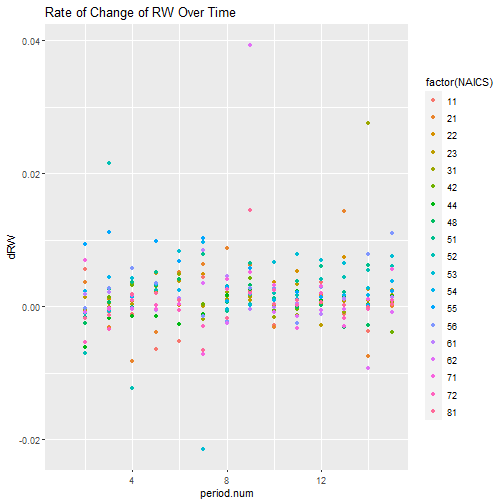
\includegraphics{Analysis-with-Interaction-Term-between-Industry-Category-and-Time--as-a-continuous-Variable-_files/figure-latex/unnamed-chunk-5-1.pdf}

However, when dummies are included, the relationship holds for some but
not for all. In the previous analysis, with only dummy variables for
industry categories, RW, OJ and PT have statistically significant
negative relationship with job reallocation rate (only RL has an
insignificant relationship). Nevertheless, with the addition of the
interaction term between industry category and time, RW, OJ and PT has
become insignificant explanations for the declining job reallocation
rate while RL becomes significant in describing it with a
\textbf{positive relationship}!

Since the \(R^2\) value increased and all of the interactive terms are
statistically significant, it is likely that idiosyncracies in the
labour market of specific industry as well as another variable that is
changing across time could better explain the trend of declining job
reallocation rate across time.

In fact, using the regression model:
\[R_{JR} = \alpha + \beta \frac{1}{T_{RL}} + \gamma t + \sum_n \delta I_n + \sum_n \lambda_n I_n t\]
* \emph{JR stands for Job Reallocation}

\begin{itemize}
\tightlist
\item
  \emph{RL stands for Required Level of Education}
\end{itemize}

gives us a better result. Which suggests that initial increase in
Required Level of Education increases the job reallocation significantly
but the effect plateaus as Required of Level of Education reaches a
point.

\begin{Shaded}
\begin{Highlighting}[]
\NormalTok{lmod <-}\StringTok{ }\KeywordTok{lm}\NormalTok{(adj_realloc }\OperatorTok{~}\StringTok{ }\KeywordTok{I}\NormalTok{(}\DecValTok{1}\OperatorTok{/}\NormalTok{RL) }\OperatorTok{+}\StringTok{ }\NormalTok{industryCategory}\OperatorTok{*}\NormalTok{period.num, t)}
\KeywordTok{summary}\NormalTok{(lmod)}
\end{Highlighting}
\end{Shaded}

\begin{verbatim}
## 
## Call:
## lm(formula = adj_realloc ~ I(1/RL) + industryCategory * period.num, 
##     data = t)
## 
## Residuals:
##      Min       1Q   Median       3Q      Max 
## -1.54514 -0.25828  0.00259  0.23165  2.12297 
## 
## Coefficients:
##                                Estimate Std. Error t value Pr(>|t|)    
## (Intercept)                    63.22984    4.86903  12.986  < 2e-16 ***
## I(1/RL)                       -49.89591   13.09851  -3.809 0.000176 ***
## industryCategory21            -35.21200    0.68293 -51.560  < 2e-16 ***
## industryCategory22            -44.67629    1.38606 -32.233  < 2e-16 ***
## industryCategory23            -20.35656    0.43496 -46.801  < 2e-16 ***
## industryCategory31            -38.64365    0.81352 -47.502  < 2e-16 ***
## industryCategory42            -38.37160    1.33950 -28.646  < 2e-16 ***
## industryCategory44            -30.08206    0.48957 -61.446  < 2e-16 ***
## industryCategory48            -33.37276    0.43723 -76.328  < 2e-16 ***
## industryCategory51            -42.45635    2.00076 -21.220  < 2e-16 ***
## industryCategory52            -41.19445    1.75743 -23.440  < 2e-16 ***
## industryCategory53            -32.83693    1.07965 -30.414  < 2e-16 ***
## industryCategory54            -39.17345    2.54929 -15.366  < 2e-16 ***
## industryCategory55            -45.51432    2.19376 -20.747  < 2e-16 ***
## industryCategory56            -27.26418    0.71818 -37.963  < 2e-16 ***
## industryCategory61            -40.63052    2.53024 -16.058  < 2e-16 ***
## industryCategory62            -44.58421    2.22252 -20.060  < 2e-16 ***
## industryCategory71            -17.26987    0.73016 -23.652  < 2e-16 ***
## industryCategory72            -23.47563    1.33319 -17.609  < 2e-16 ***
## industryCategory81            -31.94015    0.91454 -34.925  < 2e-16 ***
## period.num                     -0.69526    0.03561 -19.525  < 2e-16 ***
## industryCategory21:period.num   0.70211    0.04774  14.707  < 2e-16 ***
## industryCategory22:period.num   0.61365    0.04786  12.822  < 2e-16 ***
## industryCategory23:period.num   0.31275    0.04795   6.523 3.89e-10 ***
## industryCategory31:period.num   0.51962    0.04832  10.754  < 2e-16 ***
## industryCategory42:period.num   0.52256    0.04867  10.738  < 2e-16 ***
## industryCategory44:period.num   0.50382    0.04848  10.392  < 2e-16 ***
## industryCategory48:period.num   0.64282    0.05074  12.669  < 2e-16 ***
## industryCategory51:period.num   0.74390    0.04943  15.049  < 2e-16 ***
## industryCategory52:period.num   0.47215    0.04792   9.853  < 2e-16 ***
## industryCategory53:period.num   0.49020    0.04834  10.140  < 2e-16 ***
## industryCategory54:period.num   0.51944    0.05108  10.169  < 2e-16 ***
## industryCategory55:period.num   0.59056    0.04840  12.202  < 2e-16 ***
## industryCategory56:period.num   0.49472    0.05097   9.707  < 2e-16 ***
## industryCategory61:period.num   0.62112    0.04853  12.800  < 2e-16 ***
## industryCategory62:period.num   0.72898    0.06056  12.037  < 2e-16 ***
## industryCategory71:period.num   0.44138    0.04780   9.233  < 2e-16 ***
## industryCategory72:period.num   0.54797    0.04936  11.102  < 2e-16 ***
## industryCategory81:period.num   0.52301    0.04798  10.900  < 2e-16 ***
## ---
## Signif. codes:  0 '***' 0.001 '**' 0.01 '*' 0.05 '.' 0.1 ' ' 1
## 
## Residual standard error: 0.5647 on 246 degrees of freedom
## Multiple R-squared:  0.9958, Adjusted R-squared:  0.9952 
## F-statistic:  1539 on 38 and 246 DF,  p-value: < 2.2e-16
\end{verbatim}

\hypertarget{theoretical-explanations}{%
\subsection{Theoretical Explanations}\label{theoretical-explanations}}

A possible explanation of this phenomenon could come from the fact that
employers have little to no incentive in keeping jobs with high level of
educational requirement since investment in education is largely done by
the employee, not the employer. Hence, the costs of readjusting
employment if a mismatch occurs is lower, causing employers to be more
willing to fire employees with higher levels education.

It is also possible that mismatch occurs more frequently, given the
existence of asymmetric information for general training. Having a
degree proves that you could have the relevant skills to do the job but
it might turn out to be unsuitable for you.

Nevertheless, these explanations are also applicable to other training
indices but there is no statistically significant relationship between
them.

Using the formula
\(Job\ Reallocation = Job\ Creation + Job\ Destruction\), we can
decompose job reallocation rates to job creation rates and job
destruction rates. The following are the results on performing the
regressions using the formula below:

\[R_{job \ creation} = \alpha + \beta T_{RL} + \gamma t + \sum_n \delta I_n + \sum_n \lambda_n I_n t\]

\begin{Shaded}
\begin{Highlighting}[]
\NormalTok{lmod <-}\StringTok{ }\KeywordTok{lm}\NormalTok{(gain }\OperatorTok{~}\StringTok{ }\NormalTok{RL }\OperatorTok{+}\StringTok{ }\NormalTok{industryCategory}\OperatorTok{*}\NormalTok{period.num, t)}
\KeywordTok{summary}\NormalTok{(lmod)}
\end{Highlighting}
\end{Shaded}

\begin{verbatim}
## 
## Call:
## lm(formula = gain ~ RL + industryCategory * period.num, data = t)
## 
## Residuals:
##      Min       1Q   Median       3Q      Max 
## -2.01738 -0.17014  0.05622  0.19523  1.47606 
## 
## Coefficients:
##                                Estimate Std. Error t value Pr(>|t|)    
## (Intercept)                    23.99861    1.57120  15.274  < 2e-16 ***
## RL                             -0.62555    0.57695  -1.084    0.279    
## industryCategory21            -15.40221    0.37235 -41.365  < 2e-16 ***
## industryCategory22            -19.14362    0.66051 -28.983  < 2e-16 ***
## industryCategory23            -10.45480    0.32066 -32.604  < 2e-16 ***
## industryCategory31            -18.10197    0.41085 -44.060  < 2e-16 ***
## industryCategory42            -16.09256    0.63590 -25.307  < 2e-16 ***
## industryCategory44            -15.44940    0.32785 -47.124  < 2e-16 ***
## industryCategory48            -16.66424    0.32101 -51.912  < 2e-16 ***
## industryCategory51            -16.53787    1.09477 -15.106  < 2e-16 ***
## industryCategory52            -16.46460    0.89805 -18.334  < 2e-16 ***
## industryCategory53            -14.13947    0.51069 -27.687  < 2e-16 ***
## industryCategory54            -12.63811    1.69515  -7.455 1.53e-12 ***
## industryCategory55            -17.33412    1.27633 -13.581  < 2e-16 ***
## industryCategory56            -12.13659    0.38211 -31.762  < 2e-16 ***
## industryCategory61            -13.29794    1.66987  -7.963 6.19e-14 ***
## industryCategory62            -16.43786    1.29538 -12.690  < 2e-16 ***
## industryCategory71             -7.29498    0.38547 -18.925  < 2e-16 ***
## industryCategory72            -14.31883    0.45284 -31.620  < 2e-16 ***
## industryCategory81            -14.06003    0.44526 -31.577  < 2e-16 ***
## period.num                     -0.31380    0.02521 -12.446  < 2e-16 ***
## industryCategory21:period.num   0.25509    0.03526   7.235 5.89e-12 ***
## industryCategory22:period.num   0.28895    0.03527   8.192 1.41e-14 ***
## industryCategory23:period.num   0.21096    0.03529   5.978 7.91e-09 ***
## industryCategory31:period.num   0.27313    0.03532   7.734 2.68e-13 ***
## industryCategory42:period.num   0.24034    0.03536   6.798 7.99e-11 ***
## industryCategory44:period.num   0.22158    0.03538   6.264 1.67e-09 ***
## industryCategory48:period.num   0.31335    0.03570   8.776 2.89e-16 ***
## industryCategory51:period.num   0.34989    0.03563   9.821  < 2e-16 ***
## industryCategory52:period.num   0.23267    0.03530   6.592 2.63e-10 ***
## industryCategory53:period.num   0.24155    0.03530   6.842 6.16e-11 ***
## industryCategory54:period.num   0.20089    0.03750   5.356 1.95e-07 ***
## industryCategory55:period.num   0.28637    0.03525   8.123 2.21e-14 ***
## industryCategory56:period.num   0.20500    0.03583   5.721 3.06e-08 ***
## industryCategory61:period.num   0.26806    0.03525   7.604 6.07e-13 ***
## industryCategory62:period.num   0.25333    0.04450   5.693 3.55e-08 ***
## industryCategory71:period.num   0.22945    0.03525   6.509 4.22e-10 ***
## industryCategory72:period.num   0.24619    0.03548   6.938 3.49e-11 ***
## industryCategory81:period.num   0.25515    0.03526   7.236 5.86e-12 ***
## ---
## Signif. codes:  0 '***' 0.001 '**' 0.01 '*' 0.05 '.' 0.1 ' ' 1
## 
## Residual standard error: 0.4171 on 246 degrees of freedom
## Multiple R-squared:  0.9909, Adjusted R-squared:  0.9895 
## F-statistic: 704.9 on 38 and 246 DF,  p-value: < 2.2e-16
\end{verbatim}

\[R_{job \ destruction} = \alpha + \beta T_{RL} + \gamma t + \sum_n \delta I_n + \sum_n \lambda_n I_n t\]

\begin{Shaded}
\begin{Highlighting}[]
\NormalTok{lmod <-}\StringTok{ }\KeywordTok{lm}\NormalTok{(loss }\OperatorTok{~}\StringTok{ }\NormalTok{RL }\OperatorTok{+}\StringTok{ }\NormalTok{industryCategory}\OperatorTok{*}\NormalTok{period.num, t)}
\KeywordTok{summary}\NormalTok{(lmod)}
\end{Highlighting}
\end{Shaded}

\begin{verbatim}
## 
## Call:
## lm(formula = loss ~ RL + industryCategory * period.num, data = t)
## 
## Residuals:
##     Min      1Q  Median      3Q     Max 
## -1.6385 -0.2431 -0.0572  0.1451  4.0756 
## 
## Coefficients:
##                                Estimate Std. Error t value Pr(>|t|)    
## (Intercept)                    14.43999    2.32989   6.198 2.40e-09 ***
## RL                              2.95619    0.85555   3.455 0.000647 ***
## industryCategory21            -18.56644    0.55214 -33.626  < 2e-16 ***
## industryCategory22            -22.85114    0.97945 -23.331  < 2e-16 ***
## industryCategory23             -9.82623    0.47550 -20.665  < 2e-16 ***
## industryCategory31            -18.95866    0.60924 -31.119  < 2e-16 ***
## industryCategory42            -19.67026    0.94297 -20.860  < 2e-16 ***
## industryCategory44            -15.21776    0.48616 -31.302  < 2e-16 ***
## industryCategory48            -16.57544    0.47601 -34.821  < 2e-16 ***
## industryCategory51            -22.70704    1.62341 -13.987  < 2e-16 ***
## industryCategory52            -21.63140    1.33170 -16.243  < 2e-16 ***
## industryCategory53            -16.53757    0.75728 -21.838  < 2e-16 ***
## industryCategory54            -23.69023    2.51370  -9.424  < 2e-16 ***
## industryCategory55            -24.97925    1.89264 -13.198  < 2e-16 ***
## industryCategory56            -13.78801    0.56663 -24.334  < 2e-16 ***
## industryCategory61            -24.45710    2.47622  -9.877  < 2e-16 ***
## industryCategory62            -24.91310    1.92088 -12.970  < 2e-16 ***
## industryCategory71             -8.60294    0.57160 -15.051  < 2e-16 ***
## industryCategory72            -12.66654    0.67151 -18.863  < 2e-16 ***
## industryCategory81            -16.06199    0.66026 -24.327  < 2e-16 ***
## period.num                     -0.35344    0.03739  -9.454  < 2e-16 ***
## industryCategory21:period.num   0.44041    0.05228   8.424 3.06e-15 ***
## industryCategory22:period.num   0.30646    0.05230   5.859 1.48e-08 ***
## industryCategory23:period.num   0.11269    0.05233   2.153 0.032266 *  
## industryCategory31:period.num   0.22624    0.05237   4.320 2.26e-05 ***
## industryCategory42:period.num   0.25688    0.05243   4.900 1.74e-06 ***
## industryCategory44:period.num   0.26161    0.05246   4.987 1.16e-06 ***
## industryCategory48:period.num   0.28670    0.05294   5.415 1.46e-07 ***
## industryCategory51:period.num   0.36574    0.05283   6.923 3.82e-11 ***
## industryCategory52:period.num   0.21583    0.05234   4.123 5.11e-05 ***
## industryCategory53:period.num   0.22694    0.05235   4.335 2.13e-05 ***
## industryCategory54:period.num   0.30091    0.05561   5.411 1.49e-07 ***
## industryCategory55:period.num   0.27492    0.05228   5.259 3.15e-07 ***
## industryCategory56:period.num   0.24748    0.05313   4.658 5.23e-06 ***
## industryCategory61:period.num   0.32070    0.05228   6.135 3.39e-09 ***
## industryCategory62:period.num   0.44334    0.06599   6.718 1.27e-10 ***
## industryCategory71:period.num   0.20200    0.05228   3.864 0.000143 ***
## industryCategory72:period.num   0.27013    0.05262   5.134 5.77e-07 ***
## industryCategory81:period.num   0.25203    0.05229   4.820 2.52e-06 ***
## ---
## Signif. codes:  0 '***' 0.001 '**' 0.01 '*' 0.05 '.' 0.1 ' ' 1
## 
## Residual standard error: 0.6185 on 246 degrees of freedom
## Multiple R-squared:  0.9803, Adjusted R-squared:  0.9773 
## F-statistic: 322.3 on 38 and 246 DF,  p-value: < 2.2e-16
\end{verbatim}

The results show that the main factor behind the positive relationship
observed between RL and job reallocation rate is job destruction rate
and not job creation rate. This is a little baffling given the general
consensus in empirical evidences that the US workforce as a whole is
increasingly educated and that employers are looking for highly educated
employees.

Nevertheless, most studies look at the labour market as a whole whilst
this does not take into account the compositional shift of industries in
the economy, only the required level of education of jobs within
industries.

\hypertarget{worker-reallocation-rate}{%
\section{Worker Reallocation Rate}\label{worker-reallocation-rate}}

Worker Reallocation refers to the sum of job finding and separations, it
is a common measure of labour market fluidity because it tracks not only
the creation and destruction of jobs, but also the flow of workers
unexplained by job creation and destruction.

Worker reallocation rate is defined as worker reallocation divided by
the labour force. The data is collected from JOLTS (Job Openings and
Labour Turnover Surveys), which has monthly data on job finding and
separations.

For separations, JOLTS categorize them into layoffs and discharges,
quits and other separations. This could help us further identify the
patterns within the labor market.

\hypertarget{results-1}{%
\subsection{Results}\label{results-1}}

A multiplicative inverse model is used in this analysis as it yields a
better R-squared value.

\hypertarget{in-planton-site-training-pt-1}{%
\subsubsection{In-Plant/On-Site Training
(PT)}\label{in-planton-site-training-pt-1}}

\begin{Shaded}
\begin{Highlighting}[]
\NormalTok{lmod <-}\StringTok{ }\KeywordTok{lm}\NormalTok{(realloc_rate }\OperatorTok{~}\StringTok{ }\KeywordTok{I}\NormalTok{(}\DecValTok{1}\OperatorTok{/}\NormalTok{PT) }\OperatorTok{+}\StringTok{ }\NormalTok{industryCategoryWR}\OperatorTok{*}\NormalTok{period.num, p)}
\KeywordTok{summary}\NormalTok{(lmod)}
\end{Highlighting}
\end{Shaded}

\begin{verbatim}
## 
## Call:
## lm(formula = realloc_rate ~ I(1/PT) + industryCategoryWR * period.num, 
##     data = p)
## 
## Residuals:
##     Min      1Q  Median      3Q     Max 
## -32.462  -4.630   0.686   4.974  21.021 
## 
## Coefficients:
##                                  Estimate Std. Error t value Pr(>|t|)    
## (Intercept)                      328.5502    86.4591   3.800 0.000194 ***
## I(1/PT)                         -902.4539   308.2838  -2.927 0.003827 ** 
## industryCategoryWR23              39.4838    15.3701   2.569 0.010954 *  
## industryCategoryWR31               4.4583     9.1365   0.488 0.626125    
## industryCategoryWR42              19.4955    12.0366   1.620 0.106923    
## industryCategoryWR44             109.7884    24.0581   4.563 8.91e-06 ***
## industryCategoryWR48              38.8721    15.1774   2.561 0.011192 *  
## industryCategoryWR51               7.6660    10.4618   0.733 0.464587    
## industryCategoryWR52              19.3143    14.4783   1.334 0.183764    
## industryCategoryWR53              51.0669    12.0715   4.230 3.59e-05 ***
## industryCategoryWR54              60.4674     8.3670   7.227 1.11e-11 ***
## industryCategoryWR61              12.0016    11.8770   1.010 0.313520    
## industryCategoryWR62              64.0249    26.5033   2.416 0.016631 *  
## industryCategoryWR71             161.7785    26.6436   6.072 6.53e-09 ***
## industryCategoryWR72             208.7100    45.2324   4.614 7.16e-06 ***
## industryCategoryWR81              50.1238    15.3337   3.269 0.001277 ** 
## period.num                         1.6655     0.5359   3.108 0.002168 ** 
## industryCategoryWR23:period.num   -4.0821     0.7567  -5.395 1.99e-07 ***
## industryCategoryWR31:period.num   -2.5051     0.7658  -3.271 0.001266 ** 
## industryCategoryWR42:period.num   -2.7256     0.7612  -3.581 0.000433 ***
## industryCategoryWR44:period.num   -2.8006     0.7614  -3.678 0.000304 ***
## industryCategoryWR48:period.num   -1.3199     0.7580  -1.741 0.083225 .  
## industryCategoryWR51:period.num   -0.8698     0.7570  -1.149 0.251973    
## industryCategoryWR52:period.num   -2.9463     0.7908  -3.726 0.000255 ***
## industryCategoryWR53:period.num   -4.2507     0.7973  -5.332 2.69e-07 ***
## industryCategoryWR54:period.num   -1.1460     0.7598  -1.508 0.133094    
## industryCategoryWR61:period.num   -1.7726     0.7607  -2.330 0.020818 *  
## industryCategoryWR62:period.num   -3.0029     0.8954  -3.354 0.000959 ***
## industryCategoryWR71:period.num   -1.9256     0.7704  -2.499 0.013273 *  
## industryCategoryWR72:period.num   -2.6741     0.7589  -3.524 0.000531 ***
## industryCategoryWR81:period.num   -1.9341     0.7588  -2.549 0.011582 *  
## ---
## Signif. codes:  0 '***' 0.001 '**' 0.01 '*' 0.05 '.' 0.1 ' ' 1
## 
## Residual standard error: 8.952 on 194 degrees of freedom
## Multiple R-squared:  0.9455, Adjusted R-squared:  0.9371 
## F-statistic: 112.2 on 30 and 194 DF,  p-value: < 2.2e-16
\end{verbatim}

\hypertarget{on-the-job-training-oj-1}{%
\subsubsection{On-the-Job Training
(OJ)}\label{on-the-job-training-oj-1}}

\begin{Shaded}
\begin{Highlighting}[]
\NormalTok{lmod <-}\StringTok{ }\KeywordTok{lm}\NormalTok{(realloc_rate }\OperatorTok{~}\StringTok{ }\KeywordTok{I}\NormalTok{(}\DecValTok{1}\OperatorTok{/}\NormalTok{OJ}\OperatorTok{^}\DecValTok{5}\NormalTok{) }\OperatorTok{+}\StringTok{ }\NormalTok{industryCategoryWR}\OperatorTok{*}\NormalTok{period.num, p)}
\KeywordTok{summary}\NormalTok{(lmod)}
\end{Highlighting}
\end{Shaded}

\begin{verbatim}
## 
## Call:
## lm(formula = realloc_rate ~ I(1/OJ^5) + industryCategoryWR * 
##     period.num, data = p)
## 
## Residuals:
##      Min       1Q   Median       3Q      Max 
## -29.1222  -4.8871   0.7607   5.2096  19.9591 
## 
## Coefficients:
##                                   Estimate Std. Error t value Pr(>|t|)    
## (Intercept)                      1.362e+02  1.384e+01   9.843  < 2e-16 ***
## I(1/OJ^5)                       -6.399e+04  1.380e+04  -4.638 6.45e-06 ***
## industryCategoryWR23             4.971e+01  9.291e+00   5.350 2.46e-07 ***
## industryCategoryWR31             1.466e+01  8.967e+00   1.635 0.103702    
## industryCategoryWR42             6.098e+01  1.658e+01   3.678 0.000304 ***
## industryCategoryWR44             2.026e+02  3.521e+01   5.756 3.32e-08 ***
## industryCategoryWR48             1.039e+02  2.352e+01   4.417 1.66e-05 ***
## industryCategoryWR51             3.206e+01  1.222e+01   2.625 0.009363 ** 
## industryCategoryWR52             3.748e+01  1.369e+01   2.738 0.006765 ** 
## industryCategoryWR53             6.245e+01  1.097e+01   5.691 4.61e-08 ***
## industryCategoryWR54             5.481e+01  6.904e+00   7.939 1.60e-13 ***
## industryCategoryWR61             4.901e+01  1.559e+01   3.144 0.001928 ** 
## industryCategoryWR62             1.436e+02  3.398e+01   4.227 3.64e-05 ***
## industryCategoryWR71             3.047e+02  4.753e+01   6.411 1.08e-09 ***
## industryCategoryWR72             6.341e+02  1.201e+02   5.279 3.46e-07 ***
## industryCategoryWR81             7.162e+01  1.486e+01   4.818 2.91e-06 ***
## period.num                       1.248e+00  5.233e-01   2.384 0.018073 *  
## industryCategoryWR23:period.num -3.703e+00  7.370e-01  -5.024 1.14e-06 ***
## industryCategoryWR31:period.num -2.501e+00  7.372e-01  -3.392 0.000841 ***
## industryCategoryWR42:period.num -2.800e+00  7.367e-01  -3.801 0.000193 ***
## industryCategoryWR44:period.num -2.615e+00  7.336e-01  -3.564 0.000460 ***
## industryCategoryWR48:period.num -3.185e-01  7.567e-01  -0.421 0.674281    
## industryCategoryWR51:period.num -2.197e+00  7.817e-01  -2.811 0.005449 ** 
## industryCategoryWR52:period.num -3.531e+00  7.821e-01  -4.515 1.10e-05 ***
## industryCategoryWR53:period.num -4.126e+00  7.452e-01  -5.537 9.92e-08 ***
## industryCategoryWR54:period.num -1.523e+00  7.344e-01  -2.073 0.039455 *  
## industryCategoryWR61:period.num -1.910e+00  7.378e-01  -2.589 0.010358 *  
## industryCategoryWR62:period.num -4.758e-01  7.725e-01  -0.616 0.538713    
## industryCategoryWR71:period.num -2.459e+00  7.621e-01  -3.227 0.001468 ** 
## industryCategoryWR72:period.num -2.132e+00  7.496e-01  -2.844 0.004937 ** 
## industryCategoryWR81:period.num -1.720e+00  7.335e-01  -2.345 0.020050 *  
## ---
## Signif. codes:  0 '***' 0.001 '**' 0.01 '*' 0.05 '.' 0.1 ' ' 1
## 
## Residual standard error: 8.679 on 194 degrees of freedom
## Multiple R-squared:  0.9488, Adjusted R-squared:  0.9408 
## F-statistic: 119.8 on 30 and 194 DF,  p-value: < 2.2e-16
\end{verbatim}

\hypertarget{relevant-work-experience-rw-1}{%
\subsubsection{Relevant Work Experience
(RW)}\label{relevant-work-experience-rw-1}}

\begin{Shaded}
\begin{Highlighting}[]
\NormalTok{lmod <-}\StringTok{ }\KeywordTok{lm}\NormalTok{(realloc_rate }\OperatorTok{~}\StringTok{ }\KeywordTok{I}\NormalTok{(}\DecValTok{1}\OperatorTok{/}\NormalTok{RW}\OperatorTok{^}\DecValTok{5}\NormalTok{) }\OperatorTok{+}\StringTok{ }\NormalTok{industryCategoryWR}\OperatorTok{*}\NormalTok{period.num, p)}
\KeywordTok{summary}\NormalTok{(lmod)}
\end{Highlighting}
\end{Shaded}

\begin{verbatim}
## 
## Call:
## lm(formula = realloc_rate ~ I(1/RW^5) + industryCategoryWR * 
##     period.num, data = p)
## 
## Residuals:
##     Min      1Q  Median      3Q     Max 
## -33.996  -5.140   1.059   4.607  22.907 
## 
## Coefficients:
##                                   Estimate Std. Error t value Pr(>|t|)    
## (Intercept)                      1.237e+02  1.158e+01  10.679  < 2e-16 ***
## I(1/RW^5)                       -2.185e+05  4.829e+04  -4.525 1.05e-05 ***
## industryCategoryWR23             6.589e+01  7.350e+00   8.965 2.62e-16 ***
## industryCategoryWR31            -1.613e+00  7.154e+00  -0.225 0.821888    
## industryCategoryWR42            -1.519e+01  6.805e+00  -2.231 0.026805 *  
## industryCategoryWR44             1.761e+02  3.032e+01   5.808 2.55e-08 ***
## industryCategoryWR48             7.405e+01  1.783e+01   4.153 4.91e-05 ***
## industryCategoryWR51            -2.837e+01  7.273e+00  -3.900 0.000132 ***
## industryCategoryWR52            -1.557e+01  6.706e+00  -2.321 0.021322 *  
## industryCategoryWR53             4.157e+01  7.959e+00   5.223 4.51e-07 ***
## industryCategoryWR54             2.188e+01  8.623e+00   2.537 0.011954 *  
## industryCategoryWR61             8.740e-01  7.692e+00   0.114 0.909659    
## industryCategoryWR62             6.760e+01  1.859e+01   3.636 0.000355 ***
## industryCategoryWR71             1.582e+02  1.721e+01   9.191  < 2e-16 ***
## industryCategoryWR72             4.611e+02  8.497e+01   5.427 1.70e-07 ***
## industryCategoryWR81             3.513e+01  8.691e+00   4.043 7.62e-05 ***
## period.num                       1.123e+00  5.293e-01   2.121 0.035166 *  
## industryCategoryWR23:period.num -3.764e+00  7.377e-01  -5.103 7.93e-07 ***
## industryCategoryWR31:period.num -2.270e+00  7.357e-01  -3.085 0.002332 ** 
## industryCategoryWR42:period.num -2.283e+00  7.365e-01  -3.100 0.002223 ** 
## industryCategoryWR44:period.num -2.204e+00  7.392e-01  -2.981 0.003242 ** 
## industryCategoryWR48:period.num -1.016e+00  7.362e-01  -1.379 0.169349    
## industryCategoryWR51:period.num -1.038e+00  7.355e-01  -1.410 0.159998    
## industryCategoryWR52:period.num -2.351e+00  7.355e-01  -3.197 0.001622 ** 
## industryCategoryWR53:period.num -3.565e+00  7.353e-01  -4.848 2.55e-06 ***
## industryCategoryWR54:period.num -1.184e+00  7.362e-01  -1.608 0.109381    
## industryCategoryWR61:period.num -1.551e+00  7.353e-01  -2.109 0.036235 *  
## industryCategoryWR62:period.num -2.872e+00  7.871e-01  -3.648 0.000339 ***
## industryCategoryWR71:period.num -1.476e+00  7.353e-01  -2.007 0.046161 *  
## industryCategoryWR72:period.num -2.853e+00  7.353e-01  -3.881 0.000143 ***
## industryCategoryWR81:period.num -1.685e+00  7.355e-01  -2.290 0.023076 *  
## ---
## Signif. codes:  0 '***' 0.001 '**' 0.01 '*' 0.05 '.' 0.1 ' ' 1
## 
## Residual standard error: 8.7 on 194 degrees of freedom
## Multiple R-squared:  0.9485, Adjusted R-squared:  0.9406 
## F-statistic: 119.2 on 30 and 194 DF,  p-value: < 2.2e-16
\end{verbatim}

\hypertarget{required-level-of-education-rl-1}{%
\subsubsection{Required Level of Education
(RL)}\label{required-level-of-education-rl-1}}

\begin{Shaded}
\begin{Highlighting}[]
\NormalTok{lmod <-}\StringTok{ }\KeywordTok{lm}\NormalTok{(realloc_rate }\OperatorTok{~}\StringTok{ }\KeywordTok{I}\NormalTok{(}\DecValTok{1}\OperatorTok{/}\NormalTok{RL}\OperatorTok{^}\DecValTok{5}\NormalTok{) }\OperatorTok{+}\StringTok{ }\NormalTok{industryCategoryWR}\OperatorTok{*}\NormalTok{period.num, p)}
\KeywordTok{summary}\NormalTok{(lmod)}
\end{Highlighting}
\end{Shaded}

\begin{verbatim}
## 
## Call:
## lm(formula = realloc_rate ~ I(1/RL^5) + industryCategoryWR * 
##     period.num, data = p)
## 
## Residuals:
##     Min      1Q  Median      3Q     Max 
## -34.724  -4.902   0.543   4.664  25.805 
## 
## Coefficients:
##                                   Estimate Std. Error t value Pr(>|t|)    
## (Intercept)                      1.535e+02  1.715e+01   8.951 2.85e-16 ***
## I(1/RL^5)                       -1.964e+04  4.171e+03  -4.708 4.75e-06 ***
## industryCategoryWR23             1.355e+02  1.359e+01   9.969  < 2e-16 ***
## industryCategoryWR31            -2.643e+01  7.232e+00  -3.655 0.000331 ***
## industryCategoryWR42            -5.656e+01  1.202e+01  -4.704 4.85e-06 ***
## industryCategoryWR44             1.380e+02  2.139e+01   6.452 8.61e-10 ***
## industryCategoryWR48             5.209e+01  1.305e+01   3.993 9.27e-05 ***
## industryCategoryWR51            -8.242e+01  1.571e+01  -5.245 4.07e-07 ***
## industryCategoryWR52            -7.968e+01  1.470e+01  -5.420 1.75e-07 ***
## industryCategoryWR53            -1.135e+01  9.726e+00  -1.167 0.244810    
## industryCategoryWR54            -2.747e+01  1.707e+01  -1.609 0.109164    
## industryCategoryWR61            -9.018e+01  1.704e+01  -5.293 3.24e-07 ***
## industryCategoryWR62            -8.184e+01  1.647e+01  -4.968 1.48e-06 ***
## industryCategoryWR71             8.127e+01  6.748e+00  12.043  < 2e-16 ***
## industryCategoryWR72             4.376e+02  7.670e+01   5.705 4.29e-08 ***
## industryCategoryWR81            -1.186e+01  8.119e+00  -1.461 0.145591    
## period.num                       7.359e-01  5.474e-01   1.344 0.180439    
## industryCategoryWR23:period.num -5.212e+00  7.739e-01  -6.735 1.81e-10 ***
## industryCategoryWR31:period.num -1.611e+00  7.415e-01  -2.173 0.030998 *  
## industryCategoryWR42:period.num -1.722e+00  7.498e-01  -2.297 0.022701 *  
## industryCategoryWR44:period.num -2.182e+00  7.365e-01  -2.963 0.003426 ** 
## industryCategoryWR48:period.num  4.855e-01  8.135e-01   0.597 0.551301    
## industryCategoryWR51:period.num -8.126e-02  7.550e-01  -0.108 0.914391    
## industryCategoryWR52:period.num -1.601e+00  7.461e-01  -2.146 0.033088 *  
## industryCategoryWR53:period.num -2.878e+00  7.447e-01  -3.865 0.000152 ***
## industryCategoryWR54:period.num -4.575e-01  7.565e-01  -0.605 0.546076    
## industryCategoryWR61:period.num -7.262e-01  7.526e-01  -0.965 0.335740    
## industryCategoryWR62:period.num -2.980e-01  7.829e-01  -0.381 0.703869    
## industryCategoryWR71:period.num -1.361e+00  7.330e-01  -1.857 0.064773 .  
## industryCategoryWR72:period.num -1.581e+00  7.803e-01  -2.026 0.044126 *  
## industryCategoryWR81:period.num -1.346e+00  7.377e-01  -1.825 0.069549 .  
## ---
## Signif. codes:  0 '***' 0.001 '**' 0.01 '*' 0.05 '.' 0.1 ' ' 1
## 
## Residual standard error: 8.666 on 194 degrees of freedom
## Multiple R-squared:  0.9489, Adjusted R-squared:  0.941 
## F-statistic: 120.1 on 30 and 194 DF,  p-value: < 2.2e-16
\end{verbatim}

\hypertarget{explanations}{%
\subsection{Explanations}\label{explanations}}

Including the interaction terms with the analysis of worker reallocation
rate yields very interesting results. All of the data points to fact
that a higher training indices result to a higher worker reallocation
rate. As the exponentiation of the multiplicative inverse increases, the
higher the R-squared value (I kept the exponent at 5 for this notebook).

The consensus in existing literature is that workers with higher
training tend to have better job security and less unemployment. The
results found is counterintuitive but does not necessarily contradict
previous findings. It could be the case that workers with higher human
capital are more likely to switch jobs as they are often sought out for
their expertise. A common externality labour economists studying human
capital theory often include in their analysis is the issue of poaching
externality, whereby a company trains a worker but then the newly gained
human capital is `poached' by another firm. However, this argument
requires that the human capital observed has high generality.

It is also important to note about the assumptions behind the findings,
as well as the range of training indices changed in each industry. When
preparing the data, due to the lack of consistent time series data in
training index, the assumption of that each occupation has the same
training requirements over time. The observed difference is the
compositional shifts of occupations within the industry. The training
indices of the industry is the weighted average of the training index of
each occupation. We found that there is an increase in most industries
for most indices but the range is relatively small, at about 0.1-0.2
over the course of 15 years. Hence, the results should be not be
interpreted directly and no conclusion can be made about the effects of
training to the reallocation rates.

\hypertarget{quit-analysis}{%
\section{Quit Analysis}\label{quit-analysis}}

In the Jobs Opening and Labour Turnover Survey (JOLTS), total
separations are divided into three categories, which gives:
\[Total \ Separations = Quits \ + \ Layoffs \ and \ discharges \ + Other \ discharges \]
The relationship we are interested to look further into is the
relationship between quits and layoffs to the training indices.

Quits are seen and interpreted as voluntary discharges initiated by the
worker and not the firm. Looking at this measurement, we could analyze
the behaviour of the worker in relation to their level of training.

\hypertarget{results-2}{%
\subsection{Results}\label{results-2}}

Just like the worker reallocation rate, a multiplicative inverse model
is used for the regression.

\hypertarget{in-planton-site-training-pt-2}{%
\subsubsection{In-Plant/On-Site Training
(PT)}\label{in-planton-site-training-pt-2}}

\begin{Shaded}
\begin{Highlighting}[]
\NormalTok{lmod <-}\StringTok{ }\KeywordTok{lm}\NormalTok{(quits }\OperatorTok{~}\StringTok{ }\KeywordTok{I}\NormalTok{(}\DecValTok{1}\OperatorTok{/}\NormalTok{PT}\OperatorTok{^}\DecValTok{5}\NormalTok{) }\OperatorTok{+}\StringTok{ }\NormalTok{industryCategoryWR}\OperatorTok{*}\NormalTok{period.num, q)}
\KeywordTok{summary}\NormalTok{(lmod)}
\end{Highlighting}
\end{Shaded}

\begin{verbatim}
## 
## Call:
## lm(formula = quits ~ I(1/PT^5) + industryCategoryWR * period.num, 
##     data = q)
## 
## Residuals:
##      Min       1Q   Median       3Q      Max 
## -10.8729  -2.4142   0.2735   2.4391   9.3495 
## 
## Coefficients:
##                                   Estimate Std. Error t value Pr(>|t|)    
## (Intercept)                      2.994e+01  4.444e+00   6.737 1.79e-10 ***
## I(1/PT^5)                       -7.877e+03  2.221e+03  -3.546 0.000490 ***
## industryCategoryWR23             1.038e+00  3.893e+00   0.267 0.790078    
## industryCategoryWR31             2.711e+00  3.541e+00   0.766 0.444830    
## industryCategoryWR42             8.622e+00  4.215e+00   2.045 0.042183 *  
## industryCategoryWR44             4.745e+01  9.232e+00   5.139 6.70e-07 ***
## industryCategoryWR48             1.417e+01  5.196e+00   2.727 0.006985 ** 
## industryCategoryWR51             8.454e+00  3.823e+00   2.211 0.028184 *  
## industryCategoryWR52             1.380e+01  4.945e+00   2.791 0.005774 ** 
## industryCategoryWR53             1.773e+01  4.215e+00   4.205 3.98e-05 ***
## industryCategoryWR54             1.470e+01  3.408e+00   4.314 2.55e-05 ***
## industryCategoryWR61             6.493e+00  4.180e+00   1.553 0.121972    
## industryCategoryWR62             3.798e+01  1.059e+01   3.586 0.000425 ***
## industryCategoryWR71             4.977e+01  1.075e+01   4.628 6.73e-06 ***
## industryCategoryWR72             1.280e+02  2.718e+01   4.710 4.70e-06 ***
## industryCategoryWR81             2.296e+01  5.250e+00   4.373 1.99e-05 ***
## period.num                       6.177e-01  2.489e-01   2.482 0.013919 *  
## industryCategoryWR23:period.num -9.028e-01  3.518e-01  -2.566 0.011049 *  
## industryCategoryWR31:period.num -6.687e-01  3.531e-01  -1.894 0.059720 .  
## industryCategoryWR42:period.num -6.848e-01  3.527e-01  -1.942 0.053603 .  
## industryCategoryWR44:period.num -7.732e-01  3.538e-01  -2.186 0.030048 *  
## industryCategoryWR48:period.num -3.499e-01  3.520e-01  -0.994 0.321500    
## industryCategoryWR51:period.num -5.830e-01  3.520e-01  -1.656 0.099284 .  
## industryCategoryWR52:period.num -1.196e+00  3.604e-01  -3.320 0.001076 ** 
## industryCategoryWR53:period.num -1.253e+00  3.601e-01  -3.479 0.000622 ***
## industryCategoryWR54:period.num -9.034e-02  3.525e-01  -0.256 0.798002    
## industryCategoryWR61:period.num -5.628e-01  3.525e-01  -1.596 0.112024    
## industryCategoryWR62:period.num -1.361e+00  4.325e-01  -3.148 0.001903 ** 
## industryCategoryWR71:period.num -6.996e-01  3.600e-01  -1.943 0.053422 .  
## industryCategoryWR72:period.num -4.339e-01  3.663e-01  -1.185 0.237661    
## industryCategoryWR81:period.num -8.181e-01  3.523e-01  -2.322 0.021249 *  
## ---
## Signif. codes:  0 '***' 0.001 '**' 0.01 '*' 0.05 '.' 0.1 ' ' 1
## 
## Residual standard error: 4.163 on 194 degrees of freedom
## Multiple R-squared:  0.8425, Adjusted R-squared:  0.8181 
## F-statistic: 34.58 on 30 and 194 DF,  p-value: < 2.2e-16
\end{verbatim}

\hypertarget{on-the-job-training-oj-2}{%
\subsubsection{On-the-Job Training
(OJ)}\label{on-the-job-training-oj-2}}

\begin{Shaded}
\begin{Highlighting}[]
\NormalTok{lmod <-}\StringTok{ }\KeywordTok{lm}\NormalTok{(quits }\OperatorTok{~}\StringTok{ }\KeywordTok{I}\NormalTok{(}\DecValTok{1}\OperatorTok{/}\NormalTok{OJ}\OperatorTok{^}\DecValTok{5}\NormalTok{) }\OperatorTok{+}\StringTok{ }\NormalTok{industryCategoryWR}\OperatorTok{*}\NormalTok{period.num, q)}
\KeywordTok{summary}\NormalTok{(lmod)}
\end{Highlighting}
\end{Shaded}

\begin{verbatim}
## 
## Call:
## lm(formula = quits ~ I(1/OJ^5) + industryCategoryWR * period.num, 
##     data = q)
## 
## Residuals:
##      Min       1Q   Median       3Q      Max 
## -10.3088  -2.6148   0.4449   2.5281   9.7664 
## 
## Coefficients:
##                                   Estimate Std. Error t value Pr(>|t|)    
## (Intercept)                      4.089e+01  6.588e+00   6.208 3.20e-09 ***
## I(1/OJ^5)                       -2.600e+04  6.568e+03  -3.959 0.000106 ***
## industryCategoryWR23            -3.290e+00  4.424e+00  -0.744 0.457928    
## industryCategoryWR31             8.625e+00  4.269e+00   2.020 0.044729 *  
## industryCategoryWR42             2.749e+01  7.892e+00   3.483 0.000612 ***
## industryCategoryWR44             8.190e+01  1.676e+01   4.886 2.15e-06 ***
## industryCategoryWR48             4.215e+01  1.120e+01   3.765 0.000221 ***
## industryCategoryWR51             2.032e+01  5.816e+00   3.494 0.000589 ***
## industryCategoryWR52             2.297e+01  6.518e+00   3.524 0.000530 ***
## industryCategoryWR53             2.442e+01  5.224e+00   4.674 5.52e-06 ***
## industryCategoryWR54             1.390e+01  3.287e+00   4.229 3.61e-05 ***
## industryCategoryWR61             2.351e+01  7.421e+00   3.168 0.001785 ** 
## industryCategoryWR62             6.498e+01  1.618e+01   4.017 8.43e-05 ***
## industryCategoryWR71             1.021e+02  2.263e+01   4.511 1.12e-05 ***
## industryCategoryWR72             2.584e+02  5.718e+01   4.518 1.08e-05 ***
## industryCategoryWR81             3.324e+01  7.076e+00   4.697 4.99e-06 ***
## period.num                       4.610e-01  2.492e-01   1.850 0.065800 .  
## industryCategoryWR23:period.num -7.490e-01  3.509e-01  -2.135 0.034044 *  
## industryCategoryWR31:period.num -7.022e-01  3.510e-01  -2.001 0.046823 *  
## industryCategoryWR42:period.num -7.288e-01  3.508e-01  -2.078 0.039051 *  
## industryCategoryWR44:period.num -6.676e-01  3.493e-01  -1.911 0.057433 .  
## industryCategoryWR48:period.num  4.724e-02  3.603e-01   0.131 0.895814    
## industryCategoryWR51:period.num -1.132e+00  3.721e-01  -3.042 0.002674 ** 
## industryCategoryWR52:period.num -1.431e+00  3.723e-01  -3.842 0.000165 ***
## industryCategoryWR53:period.num -1.229e+00  3.548e-01  -3.465 0.000653 ***
## industryCategoryWR54:period.num -2.376e-01  3.497e-01  -0.679 0.497680    
## industryCategoryWR61:period.num -6.319e-01  3.512e-01  -1.799 0.073554 .  
## industryCategoryWR62:period.num -1.249e-02  3.678e-01  -0.034 0.972938    
## industryCategoryWR71:period.num -8.195e-01  3.628e-01  -2.259 0.025026 *  
## industryCategoryWR72:period.num -5.041e-01  3.569e-01  -1.413 0.159354    
## industryCategoryWR81:period.num -7.384e-01  3.492e-01  -2.114 0.035752 *  
## ---
## Signif. codes:  0 '***' 0.001 '**' 0.01 '*' 0.05 '.' 0.1 ' ' 1
## 
## Residual standard error: 4.132 on 194 degrees of freedom
## Multiple R-squared:  0.8448, Adjusted R-squared:  0.8208 
## F-statistic:  35.2 on 30 and 194 DF,  p-value: < 2.2e-16
\end{verbatim}

\hypertarget{related-work-experience-rw}{%
\subsubsection{Related Work Experience
(RW)}\label{related-work-experience-rw}}

\begin{Shaded}
\begin{Highlighting}[]
\NormalTok{lmod <-}\StringTok{ }\KeywordTok{lm}\NormalTok{(quits }\OperatorTok{~}\StringTok{ }\KeywordTok{I}\NormalTok{(}\DecValTok{1}\OperatorTok{/}\NormalTok{RW}\OperatorTok{^}\DecValTok{5}\NormalTok{) }\OperatorTok{+}\StringTok{ }\NormalTok{industryCategoryWR}\OperatorTok{*}\NormalTok{period.num, q)}
\KeywordTok{summary}\NormalTok{(lmod)}
\end{Highlighting}
\end{Shaded}

\begin{verbatim}
## 
## Call:
## lm(formula = quits ~ I(1/RW^5) + industryCategoryWR * period.num, 
##     data = q)
## 
## Residuals:
##      Min       1Q   Median       3Q      Max 
## -10.4117  -2.6528   0.3603   2.4958  10.9294 
## 
## Coefficients:
##                                   Estimate Std. Error t value Pr(>|t|)    
## (Intercept)                      3.619e+01  5.503e+00   6.577 4.36e-10 ***
## I(1/RW^5)                       -9.049e+04  2.294e+04  -3.945 0.000112 ***
## industryCategoryWR23             3.178e+00  3.492e+00   0.910 0.363916    
## industryCategoryWR31             2.102e+00  3.399e+00   0.618 0.536973    
## industryCategoryWR42            -3.503e+00  3.233e+00  -1.083 0.279990    
## industryCategoryWR44             7.216e+01  1.440e+01   5.010 1.22e-06 ***
## industryCategoryWR48             3.062e+01  8.470e+00   3.616 0.000382 ***
## industryCategoryWR51            -4.338e+00  3.455e+00  -1.256 0.210803    
## industryCategoryWR52             1.431e+00  3.186e+00   0.449 0.653738    
## industryCategoryWR53             1.609e+01  3.781e+00   4.255 3.25e-05 ***
## industryCategoryWR54             3.265e-01  4.096e+00   0.080 0.936562    
## industryCategoryWR61             4.081e+00  3.654e+00   1.117 0.265449    
## industryCategoryWR62             3.469e+01  8.833e+00   3.928 0.000119 ***
## industryCategoryWR71             4.309e+01  8.175e+00   5.270 3.61e-07 ***
## industryCategoryWR72             1.911e+02  4.037e+01   4.733 4.25e-06 ***
## industryCategoryWR81             1.861e+01  4.129e+00   4.507 1.14e-05 ***
## period.num                       4.067e-01  2.514e-01   1.617 0.107428    
## industryCategoryWR23:period.num -7.719e-01  3.504e-01  -2.203 0.028803 *  
## industryCategoryWR31:period.num -6.092e-01  3.495e-01  -1.743 0.082896 .  
## industryCategoryWR42:period.num -5.170e-01  3.499e-01  -1.478 0.141120    
## industryCategoryWR44:period.num -4.978e-01  3.512e-01  -1.418 0.157940    
## industryCategoryWR48:period.num -2.347e-01  3.497e-01  -0.671 0.502961    
## industryCategoryWR51:period.num -6.616e-01  3.494e-01  -1.893 0.059796 .  
## industryCategoryWR52:period.num -9.516e-01  3.494e-01  -2.723 0.007049 ** 
## industryCategoryWR53:period.num -1.002e+00  3.493e-01  -2.868 0.004595 ** 
## industryCategoryWR54:period.num -9.861e-02  3.497e-01  -0.282 0.778265    
## industryCategoryWR61:period.num -4.859e-01  3.493e-01  -1.391 0.165754    
## industryCategoryWR62:period.num -9.960e-01  3.739e-01  -2.664 0.008377 ** 
## industryCategoryWR71:period.num -4.194e-01  3.493e-01  -1.201 0.231283    
## industryCategoryWR72:period.num -7.974e-01  3.493e-01  -2.283 0.023516 *  
## industryCategoryWR81:period.num -7.234e-01  3.494e-01  -2.070 0.039734 *  
## ---
## Signif. codes:  0 '***' 0.001 '**' 0.01 '*' 0.05 '.' 0.1 ' ' 1
## 
## Residual standard error: 4.133 on 194 degrees of freedom
## Multiple R-squared:  0.8447, Adjusted R-squared:  0.8207 
## F-statistic: 35.18 on 30 and 194 DF,  p-value: < 2.2e-16
\end{verbatim}

\hypertarget{required-level-of-education-rl-2}{%
\subsubsection{Required Level of Education
(RL)}\label{required-level-of-education-rl-2}}

\begin{Shaded}
\begin{Highlighting}[]
\NormalTok{lmod <-}\StringTok{ }\KeywordTok{lm}\NormalTok{(quits }\OperatorTok{~}\StringTok{ }\KeywordTok{I}\NormalTok{(}\DecValTok{1}\OperatorTok{/}\NormalTok{RL}\OperatorTok{^}\DecValTok{5}\NormalTok{) }\OperatorTok{+}\StringTok{ }\NormalTok{industryCategoryWR}\OperatorTok{*}\NormalTok{period.num, q)}
\KeywordTok{summary}\NormalTok{(lmod)}
\end{Highlighting}
\end{Shaded}

\begin{verbatim}
## 
## Call:
## lm(formula = quits ~ I(1/RL^5) + industryCategoryWR * period.num, 
##     data = q)
## 
## Residuals:
##      Min       1Q   Median       3Q      Max 
## -11.3593  -2.6092   0.1124   2.6081   9.5675 
## 
## Coefficients:
##                                   Estimate Std. Error t value Pr(>|t|)    
## (Intercept)                      3.630e+01  8.368e+00   4.338 2.31e-05 ***
## I(1/RL^5)                       -5.041e+03  2.036e+03  -2.476 0.014138 *  
## industryCategoryWR23             2.322e+01  6.634e+00   3.501 0.000575 ***
## industryCategoryWR31            -6.085e+00  3.530e+00  -1.724 0.086303 .  
## industryCategoryWR42            -1.321e+01  5.868e+00  -2.252 0.025464 *  
## industryCategoryWR44             4.130e+01  1.044e+01   3.957 0.000106 ***
## industryCategoryWR48             1.321e+01  6.368e+00   2.074 0.039383 *  
## industryCategoryWR51            -1.617e+01  7.669e+00  -2.109 0.036267 *  
## industryCategoryWR52            -1.541e+01  7.174e+00  -2.147 0.033004 *  
## industryCategoryWR53            -5.738e-01  4.747e+00  -0.121 0.903899    
## industryCategoryWR54            -8.459e+00  8.330e+00  -1.015 0.311158    
## industryCategoryWR61            -2.200e+01  8.315e+00  -2.646 0.008815 ** 
## industryCategoryWR62            -1.603e+01  8.040e+00  -1.994 0.047550 *  
## industryCategoryWR71             1.204e+01  3.293e+00   3.657 0.000329 ***
## industryCategoryWR72             1.246e+02  3.743e+01   3.330 0.001039 ** 
## industryCategoryWR81             2.586e+00  3.962e+00   0.653 0.514833    
## period.num                       3.780e-01  2.672e-01   1.415 0.158684    
## industryCategoryWR23:period.num -1.186e+00  3.777e-01  -3.140 0.001952 ** 
## industryCategoryWR31:period.num -4.227e-01  3.619e-01  -1.168 0.244193    
## industryCategoryWR42:period.num -4.039e-01  3.659e-01  -1.104 0.271112    
## industryCategoryWR44:period.num -5.467e-01  3.594e-01  -1.521 0.129882    
## industryCategoryWR48:period.num  1.244e-01  3.970e-01   0.313 0.754376    
## industryCategoryWR51:period.num -4.014e-01  3.684e-01  -1.090 0.277274    
## industryCategoryWR52:period.num -7.467e-01  3.641e-01  -2.051 0.041656 *  
## industryCategoryWR53:period.num -8.174e-01  3.635e-01  -2.249 0.025641 *  
## industryCategoryWR54:period.num  6.168e-02  3.692e-01   0.167 0.867498    
## industryCategoryWR61:period.num -2.729e-01  3.673e-01  -0.743 0.458365    
## industryCategoryWR62:period.num -1.353e-01  3.821e-01  -0.354 0.723701    
## industryCategoryWR71:period.num -3.939e-01  3.577e-01  -1.101 0.272206    
## industryCategoryWR72:period.num -4.701e-01  3.808e-01  -1.234 0.218549    
## industryCategoryWR81:period.num -6.489e-01  3.600e-01  -1.802 0.073051 .  
## ---
## Signif. codes:  0 '***' 0.001 '**' 0.01 '*' 0.05 '.' 0.1 ' ' 1
## 
## Residual standard error: 4.229 on 194 degrees of freedom
## Multiple R-squared:  0.8374, Adjusted R-squared:  0.8122 
## F-statistic:  33.3 on 30 and 194 DF,  p-value: < 2.2e-16
\end{verbatim}

\hypertarget{explanations-1}{%
\subsection{Explanations}\label{explanations-1}}

The results above shows that PT, RW and OJ have a statistically
significant positive relationship with quit rates when the interactive
term is included. This means that at least part of the relationship
between these three training indices and the worker reallocation rates
can be explained by a higher rate of quits.

There could be some explanations behind the higher willingness of
workers to quit jobs with higher PT, RW and OJ. Assuming that these
three indices are considered to be human capital with higher specificity
(but not entirely specific), then it is likely that the investment is
made on the part of the firm and not the worker, and hence the yield of
the match would be obtained by the firm and not the worker. This might
result to a lower incentive for the worker to retain their jobs. Coupled
with information assymetry, whereby workers know the available wages
offered in the labour market to them while the firm does not, this could
explain why workers with these higher training indices have lower
attachment to their jobs and have a higher willingness to quit.

On the other hand, RL has no statistically significant relationship with
quit rates. This means that the observed statistically significant
relationship between RL and worker reallocation rate is influenced by
layoffs and or other discharges.

\hypertarget{layoff-analysis}{%
\section{Layoff Analysis}\label{layoff-analysis}}

Layoffs and Discharges are interpreted as separations that are initiated
by the firm, not the employee. From the employees' perspectives, such a
separation is involuntary and looking at this measurement could provide
us with insights about the employers' decision in separation with
regards to the level of training.

\hypertarget{results-3}{%
\subsection{Results}\label{results-3}}

A multiplicative inverse model is also used for the following
regressions.

\hypertarget{in-planton-site-training-pt-3}{%
\subsubsection{In-Plant/On-Site Training
(PT)}\label{in-planton-site-training-pt-3}}

\begin{Shaded}
\begin{Highlighting}[]
\NormalTok{lmod <-}\StringTok{ }\KeywordTok{lm}\NormalTok{(layoffs }\OperatorTok{~}\StringTok{ }\KeywordTok{I}\NormalTok{(}\DecValTok{1}\OperatorTok{/}\NormalTok{PT}\OperatorTok{^}\DecValTok{3}\NormalTok{) }\OperatorTok{+}\StringTok{ }\NormalTok{industryCategoryWR}\OperatorTok{*}\NormalTok{period.num, l)}
\KeywordTok{summary}\NormalTok{(lmod)}
\end{Highlighting}
\end{Shaded}

\begin{verbatim}
## 
## Call:
## lm(formula = layoffs ~ I(1/PT^3) + industryCategoryWR * period.num, 
##     data = l)
## 
## Residuals:
##      Min       1Q   Median       3Q      Max 
## -10.9251  -1.3265  -0.3001   0.7542  20.0997 
## 
## Coefficients:
##                                  Estimate Std. Error t value Pr(>|t|)    
## (Intercept)                      15.40568    8.35596   1.844 0.066756 .  
## I(1/PT^3)                       -68.79192  370.34961  -0.186 0.852836    
## industryCategoryWR23             36.14337    4.27572   8.453 6.70e-15 ***
## industryCategoryWR31              2.97587    3.26883   0.910 0.363752    
## industryCategoryWR42              2.15587    4.13960   0.521 0.603105    
## industryCategoryWR44             10.00070    8.83631   1.132 0.259127    
## industryCategoryWR48              4.28332    5.21782   0.821 0.412710    
## industryCategoryWR51             -1.62560    3.65123  -0.445 0.656657    
## industryCategoryWR52             -3.87595    4.96119  -0.781 0.435606    
## industryCategoryWR53              8.68102    4.14504   2.094 0.037531 *  
## industryCategoryWR54             15.91051    3.06833   5.185 5.40e-07 ***
## industryCategoryWR61              0.03002    4.09287   0.007 0.994155    
## industryCategoryWR62             -1.83292    9.93386  -0.185 0.853804    
## industryCategoryWR71             37.44954   10.03049   3.734 0.000248 ***
## industryCategoryWR72             14.77254   20.48612   0.721 0.471716    
## industryCategoryWR81              2.81748    5.27424   0.534 0.593818    
## period.num                        0.50811    0.21171   2.400 0.017340 *  
## industryCategoryWR23:period.num  -1.58395    0.29919  -5.294 3.22e-07 ***
## industryCategoryWR31:period.num  -0.95233    0.30124  -3.161 0.001823 ** 
## industryCategoryWR42:period.num  -0.95539    0.30036  -3.181 0.001710 ** 
## industryCategoryWR44:period.num  -1.02441    0.30098  -3.404 0.000808 ***
## industryCategoryWR48:period.num  -0.65310    0.29950  -2.181 0.030412 *  
## industryCategoryWR51:period.num  -0.36913    0.29931  -1.233 0.218968    
## industryCategoryWR52:period.num  -0.70992    0.30973  -2.292 0.022976 *  
## industryCategoryWR53:period.num  -1.19046    0.31050  -3.834 0.000170 ***
## industryCategoryWR54:period.num  -0.78313    0.30005  -2.610 0.009761 ** 
## industryCategoryWR61:period.num  -0.57577    0.30020  -1.918 0.056585 .  
## industryCategoryWR62:period.num  -0.67674    0.36401  -1.859 0.064526 .  
## industryCategoryWR71:period.num  -0.74692    0.30554  -2.445 0.015395 *  
## industryCategoryWR72:period.num  -0.92982    0.30344  -3.064 0.002492 ** 
## industryCategoryWR81:period.num  -0.43997    0.29974  -1.468 0.143766    
## ---
## Signif. codes:  0 '***' 0.001 '**' 0.01 '*' 0.05 '.' 0.1 ' ' 1
## 
## Residual standard error: 3.539 on 194 degrees of freedom
## Multiple R-squared:  0.9209, Adjusted R-squared:  0.9087 
## F-statistic: 75.32 on 30 and 194 DF,  p-value: < 2.2e-16
\end{verbatim}

\hypertarget{on-the-job-training-oj-3}{%
\subsubsection{On-the-Job Training
(OJ)}\label{on-the-job-training-oj-3}}

\begin{Shaded}
\begin{Highlighting}[]
\NormalTok{lmod <-}\StringTok{ }\KeywordTok{lm}\NormalTok{(layoffs }\OperatorTok{~}\StringTok{ }\KeywordTok{I}\NormalTok{(}\DecValTok{1}\OperatorTok{/}\NormalTok{OJ}\OperatorTok{^}\DecValTok{3}\NormalTok{) }\OperatorTok{+}\StringTok{ }\NormalTok{industryCategoryWR}\OperatorTok{*}\NormalTok{period.num, l)}
\KeywordTok{summary}\NormalTok{(lmod)}
\end{Highlighting}
\end{Shaded}

\begin{verbatim}
## 
## Call:
## lm(formula = layoffs ~ I(1/OJ^3) + industryCategoryWR * period.num, 
##     data = l)
## 
## Residuals:
##      Min       1Q   Median       3Q      Max 
## -10.9242  -1.3222  -0.3248   0.7860  20.0205 
## 
## Coefficients:
##                                  Estimate Std. Error t value Pr(>|t|)    
## (Intercept)                       26.0088    14.1858   1.833 0.068269 .  
## I(1/OJ^3)                       -791.5995   918.4863  -0.862 0.389833    
## industryCategoryWR23              32.6587     5.4748   5.965 1.14e-08 ***
## industryCategoryWR31               5.7446     4.5116   1.273 0.204434    
## industryCategoryWR42               8.7272     8.7301   1.000 0.318716    
## industryCategoryWR44              22.6951    16.7625   1.354 0.177336    
## industryCategoryWR48              13.4867    11.9508   1.129 0.260493    
## industryCategoryWR51               2.9835     6.4701   0.461 0.645224    
## industryCategoryWR52               1.1665     7.2708   0.160 0.872703    
## industryCategoryWR53              12.4674     5.7489   2.169 0.031324 *  
## industryCategoryWR54              16.6186     2.9397   5.653 5.57e-08 ***
## industryCategoryWR61               6.1628     8.2354   0.748 0.455163    
## industryCategoryWR62              10.2328    16.2867   0.628 0.530554    
## industryCategoryWR71              53.8747    21.3124   2.528 0.012273 *  
## industryCategoryWR72              47.7318    42.7049   1.118 0.265072    
## industryCategoryWR81               8.3382     7.8631   1.060 0.290271    
## period.num                         0.4667     0.2161   2.160 0.032034 *  
## industryCategoryWR23:period.num   -1.5418     0.3024  -5.099 8.09e-07 ***
## industryCategoryWR31:period.num   -0.9784     0.3010  -3.251 0.001357 ** 
## industryCategoryWR42:period.num   -0.9688     0.2994  -3.236 0.001424 ** 
## industryCategoryWR44:period.num   -1.0066     0.2989  -3.368 0.000914 ***
## industryCategoryWR48:period.num   -0.5678     0.3136  -1.811 0.071736 .  
## industryCategoryWR51:period.num   -0.4893     0.3286  -1.489 0.138092    
## industryCategoryWR52:period.num   -0.8089     0.3265  -2.477 0.014094 *  
## industryCategoryWR53:period.num   -1.2298     0.3053  -4.028 8.06e-05 ***
## industryCategoryWR54:period.num   -0.8057     0.2993  -2.692 0.007733 ** 
## industryCategoryWR61:period.num   -0.5948     0.2999  -1.984 0.048705 *  
## industryCategoryWR62:period.num   -0.5414     0.3190  -1.697 0.091300 .  
## industryCategoryWR71:period.num   -0.7808     0.3032  -2.575 0.010763 *  
## industryCategoryWR72:period.num   -0.8807     0.3062  -2.876 0.004475 ** 
## industryCategoryWR81:period.num   -0.4225     0.2990  -1.413 0.159315    
## ---
## Signif. codes:  0 '***' 0.001 '**' 0.01 '*' 0.05 '.' 0.1 ' ' 1
## 
## Residual standard error: 3.533 on 194 degrees of freedom
## Multiple R-squared:  0.9212, Adjusted R-squared:  0.909 
## F-statistic: 75.62 on 30 and 194 DF,  p-value: < 2.2e-16
\end{verbatim}

\hypertarget{related-work-experience-rw-1}{%
\subsubsection{Related Work Experience
(RW)}\label{related-work-experience-rw-1}}

\begin{Shaded}
\begin{Highlighting}[]
\NormalTok{lmod <-}\StringTok{ }\KeywordTok{lm}\NormalTok{(layoffs }\OperatorTok{~}\StringTok{ }\KeywordTok{I}\NormalTok{(}\DecValTok{1}\OperatorTok{/}\NormalTok{RW}\OperatorTok{^}\DecValTok{3}\NormalTok{) }\OperatorTok{+}\StringTok{ }\NormalTok{industryCategoryWR}\OperatorTok{*}\NormalTok{period.num, l)}
\KeywordTok{summary}\NormalTok{(lmod)}
\end{Highlighting}
\end{Shaded}

\begin{verbatim}
## 
## Call:
## lm(formula = layoffs ~ I(1/RW^3) + industryCategoryWR * period.num, 
##     data = l)
## 
## Residuals:
##      Min       1Q   Median       3Q      Max 
## -10.9002  -1.3309  -0.2962   0.8341  20.0694 
## 
## Coefficients:
##                                  Estimate Std. Error t value Pr(>|t|)    
## (Intercept)                       19.8472    11.0392   1.798 0.073750 .  
## I(1/RW^3)                       -933.5677  1705.0573  -0.548 0.584645    
## industryCategoryWR23              35.6529     3.3834  10.538  < 2e-16 ***
## industryCategoryWR31               3.4648     3.1083   1.115 0.266359    
## industryCategoryWR42               1.1325     2.8361   0.399 0.690100    
## industryCategoryWR44              15.7312    13.5927   1.157 0.248564    
## industryCategoryWR48               7.9671     8.6754   0.918 0.359573    
## industryCategoryWR51              -3.1003     3.2973  -0.940 0.348261    
## industryCategoryWR52              -4.4670     2.7376  -1.632 0.104367    
## industryCategoryWR53               9.4584     3.6800   2.570 0.010913 *  
## industryCategoryWR54              13.5512     4.6941   2.887 0.004332 ** 
## industryCategoryWR61               0.6646     3.4945   0.190 0.849370    
## industryCategoryWR62               1.1023     9.0213   0.122 0.902874    
## industryCategoryWR71              40.0118     8.4064   4.760 3.78e-06 ***
## industryCategoryWR72              27.2947    29.8826   0.913 0.362167    
## industryCategoryWR81               3.6905     4.1435   0.891 0.374206    
## period.num                         0.4718     0.2206   2.138 0.033731 *  
## industryCategoryWR23:period.num   -1.5637     0.3010  -5.196 5.14e-07 ***
## industryCategoryWR31:period.num   -0.9510     0.2991  -3.180 0.001716 ** 
## industryCategoryWR42:period.num   -0.9359     0.3001  -3.119 0.002093 ** 
## industryCategoryWR44:period.num   -0.9881     0.3040  -3.251 0.001357 ** 
## industryCategoryWR48:period.num   -0.6303     0.3012  -2.093 0.037675 *  
## industryCategoryWR51:period.num   -0.3849     0.3000  -1.283 0.200987    
## industryCategoryWR52:period.num   -0.7004     0.2991  -2.342 0.020200 *  
## industryCategoryWR53:period.num   -1.1741     0.2989  -3.928 0.000119 ***
## industryCategoryWR54:period.num   -0.7821     0.2991  -2.615 0.009626 ** 
## industryCategoryWR61:period.num   -0.5673     0.2990  -1.897 0.059287 .  
## industryCategoryWR62:period.num   -0.6948     0.3163  -2.197 0.029226 *  
## industryCategoryWR71:period.num   -0.7230     0.2998  -2.412 0.016813 *  
## industryCategoryWR72:period.num   -0.9187     0.3013  -3.049 0.002614 ** 
## industryCategoryWR81:period.num   -0.4256     0.2996  -1.421 0.157034    
## ---
## Signif. codes:  0 '***' 0.001 '**' 0.01 '*' 0.05 '.' 0.1 ' ' 1
## 
## Residual standard error: 3.537 on 194 degrees of freedom
## Multiple R-squared:  0.921,  Adjusted R-squared:  0.9088 
## F-statistic: 75.43 on 30 and 194 DF,  p-value: < 2.2e-16
\end{verbatim}

\hypertarget{required-level-of-education-rl-3}{%
\subsubsection{Required Level of Education
(RL)}\label{required-level-of-education-rl-3}}

\begin{Shaded}
\begin{Highlighting}[]
\NormalTok{lmod <-}\StringTok{ }\KeywordTok{lm}\NormalTok{(layoffs }\OperatorTok{~}\StringTok{ }\KeywordTok{I}\NormalTok{(}\DecValTok{1}\OperatorTok{/}\NormalTok{RL}\OperatorTok{^}\DecValTok{3}\NormalTok{) }\OperatorTok{+}\StringTok{ }\NormalTok{industryCategoryWR}\OperatorTok{*}\NormalTok{period.num, l)}
\KeywordTok{summary}\NormalTok{(lmod)}
\end{Highlighting}
\end{Shaded}

\begin{verbatim}
## 
## Call:
## lm(formula = layoffs ~ I(1/RL^3) + industryCategoryWR * period.num, 
##     data = l)
## 
## Residuals:
##     Min      1Q  Median      3Q     Max 
## -9.8211 -1.2893 -0.2686  0.7940 19.5513 
## 
## Coefficients:
##                                   Estimate Std. Error t value Pr(>|t|)    
## (Intercept)                      5.622e+01  1.246e+01   4.510 1.12e-05 ***
## I(1/RL^3)                       -1.170e+03  3.408e+02  -3.434 0.000727 ***
## industryCategoryWR23             5.304e+01  5.427e+00   9.773  < 2e-16 ***
## industryCategoryWR31            -1.884e+00  2.951e+00  -0.638 0.523923    
## industryCategoryWR42            -1.660e+01  5.916e+00  -2.807 0.005518 ** 
## industryCategoryWR44             3.463e+01  8.070e+00   4.291 2.81e-05 ***
## industryCategoryWR48             1.892e+01  5.220e+00   3.624 0.000370 ***
## industryCategoryWR51            -3.160e+01  8.992e+00  -3.514 0.000550 ***
## industryCategoryWR52            -3.060e+01  8.006e+00  -3.822 0.000178 ***
## industryCategoryWR53            -4.022e+00  4.408e+00  -0.912 0.362745    
## industryCategoryWR54            -1.994e+01  1.069e+01  -1.865 0.063735 .  
## industryCategoryWR61            -3.595e+01  1.065e+01  -3.377 0.000884 ***
## industryCategoryWR62            -3.605e+01  9.808e+00  -3.675 0.000307 ***
## industryCategoryWR71             3.394e+01  2.688e+00  12.625  < 2e-16 ***
## industryCategoryWR72             8.805e+01  2.259e+01   3.898 0.000134 ***
## industryCategoryWR81            -5.646e+00  3.450e+00  -1.636 0.103363    
## period.num                       2.216e-01  2.215e-01   1.000 0.318428    
## industryCategoryWR23:period.num -1.853e+00  3.009e-01  -6.158 4.17e-09 ***
## industryCategoryWR31:period.num -7.634e-01  2.953e-01  -2.585 0.010460 *  
## industryCategoryWR42:period.num -7.027e-01  2.993e-01  -2.348 0.019878 *  
## industryCategoryWR44:period.num -8.461e-01  2.948e-01  -2.871 0.004551 ** 
## industryCategoryWR48:period.num -1.493e-01  3.251e-01  -0.459 0.646531    
## industryCategoryWR51:period.num -6.636e-02  3.037e-01  -0.219 0.827264    
## industryCategoryWR52:period.num -5.155e-01  2.951e-01  -1.747 0.082259 .  
## industryCategoryWR53:period.num -9.737e-01  2.963e-01  -3.286 0.001206 ** 
## industryCategoryWR54:period.num -4.413e-01  3.075e-01  -1.435 0.152765    
## industryCategoryWR61:period.num -3.087e-01  3.003e-01  -1.028 0.305371    
## industryCategoryWR62:period.num -1.317e-02  3.428e-01  -0.038 0.969401    
## industryCategoryWR71:period.num -6.908e-01  2.908e-01  -2.376 0.018484 *  
## industryCategoryWR72:period.num -5.834e-01  3.084e-01  -1.892 0.060001 .  
## industryCategoryWR81:period.num -3.118e-01  2.927e-01  -1.065 0.288112    
## ---
## Signif. codes:  0 '***' 0.001 '**' 0.01 '*' 0.05 '.' 0.1 ' ' 1
## 
## Residual standard error: 3.437 on 194 degrees of freedom
## Multiple R-squared:  0.9255, Adjusted R-squared:  0.9139 
## F-statistic: 80.28 on 30 and 194 DF,  p-value: < 2.2e-16
\end{verbatim}

\hypertarget{explanations-2}{%
\subsection{Explanations}\label{explanations-2}}

Interestingly, layoffs and discharges have no statistically significant
relationship with OJ, PT and RW but instead, have a positive
relationship with RL. This means that it is likely that the observed
relationship in worker reallocation rate is dominated by quits for OJ,
PT and RW whereas RL is better explained by layoffs.

The results concur with the dataset in the Business Employment Dynamics,
whereby the observed relationship between RL and Job Reallocation Rate
is primarily driven by Job Destruction. Consequentially, layoffs is the
primary factor behind the relationship between worker reallocation rate
and RL.

\end{document}
